% MSc dissertation example file, February 2022
%
% Leave one of the documentclass lines uncommented to match your degree.
% You may remove the logo option if it causes problems.
% Do not change any other options.
% \documentclass[logo,msc,adi]{infthesis}     % Adv Design Inf
% \documentclass[logo,msc,ai]{infthesis}      % AI
% \documentclass[logo,msc,cogsci]{infthesis}  % Cognitive Sci
% \documentclass[logo,msc,cs]{infthesis}      % Computer Sci
% \documentclass[logo,msc,cyber]{infthesis}   % Cyber Sec
% \documentclass[logo,msc,datasci]{infthesis} % Data Sci
% \documentclass[logo,msc,di]{infthesis}      % Design Inf
\documentclass[logo,msc,dsti]{infthesis}    % Data Sci TI
% \documentclass[logo,msc,inf]{infthesis}     % Informatics
% \documentclass[logo,msc]{infthesis}           % degree unspecified, do not change except to add your degree
%%%%%%%%%%%%%%%%%%%%%%%%
% Understand any problems and seek approval before assuming it's ok to remove ugcheck.
\usepackage{msccheck}

% Include any packages you need below, but don't include any that change the page
% layout or style of the dissertation. By including the ugcheck package above,
% you should catch most accidental changes of page layout though.

\usepackage{microtype} % recommended, but you can remove if it causes problems
\usepackage{caption}
\usepackage{subcaption}
\usepackage{url}
\usepackage{hyperref}
\usepackage{graphicx}
\usepackage{xcolor}
\usepackage{gnuplottex}
\usepackage{tikz}
\usetikzlibrary{arrows}
\usetikzlibrary{calc}
\usetikzlibrary{positioning}
\usepackage{svg}
\usepackage{pdfpages}
\usepackage{listings}
\usepackage[ruled]{algorithm2e}

\hypersetup{colorlinks=true,linkcolor=blue,filecolor=blue,urlcolor=blue,citecolor=blue}


\begin{document}
\begin{preliminary}

\title{OpenTTDLab: A framework for repeatable, Replicable, \& Reproducible experiments using OpenTTD}

\author{Michal Charemza}

\date{\today}

\abstract{
OpenTTD is an open source business simulation game based on the 1994 game Transport Tycoon Deluxe, and in spite of being designed for recreation, OpenTTD has been used in a number of academic studies. However, these studies have problems regarding the repeatability, replicability, \& reproducibility of their experiments. In this dissertation, I present OpenTTDLab, a framework I created that allows OpenTTD to be used in a way that avoids these problems. I then show proof-of-concept results using this framework that I argue are repeatable, replicable, and reproducible; thus, giving evidence that OpenTTDLab can be a useful tool in future research.
}

\maketitle

\newenvironment{ethics}
   {\begin{frontenv}{Research Ethics Approval}{\LARGE}}
   {\end{frontenv}\newpage}

\begin{ethics}
This project was planned in accordance with the Informatics Research
Ethics policy. It did not involve any aspects that required approval
from the Informatics Research Ethics committee.

\standarddeclaration
\end{ethics}


\begin{acknowledgements}

Firstly thank you to Chris Sawyer, the original author of Transport Tycoon Deluxe: without you this project would not have existed. Then of course thank you to all the contributors of OpenTTLab over its 20 year history. And of these, thank you especially to Patric Stout (A.K.A. Truebrain), who not only gave advice and what I interpreted to be light blessing to this project, but also wrote the OpenTTD save game parser that OpenTTDLab originally forked from.

Thank you also to Ian Earle (A.K.A. BasicBeluga) who found an issue in the documentation of OpenTTDLab and submitted a fix for it. While this was a small change, I took it as evidence that what I was creating stood a chance of being useful, and pushed me to continue.

Thank you to my supervisor Michael Hermann. His ongoing advice throughout this project has been invaluable, and I think also pushed me to do as good a job as I can, including making sure that I have some results to show and discuss, and didn't get too lost in just making OpenTTDLab. This project had a few incarnations, and I think him especially for keeping any frustrations with me inside!

Of course thank you to my husband Matthew Beach, an amazingly loving and supportive partner, and whose support and advice throughout this project has been beyond invaluable. And finally, thank you to our dog, Elliot: he's a good boy.

\end{acknowledgements}


\tableofcontents
\end{preliminary}


\chapter{Introduction}

OpenTTD \cite{openttd} is an open source real time strategy (RTS) simulation game based on the 1994 game Transport Tycoon Deluxe by Chris Sawyer. The aim of the game is to successfully run a business by constructing networks of roads, railways, airports and ports, along with their respective vehicles, trains, planes and ships, in order to transport people and goods in exchange for money. OpenTTD is played on a simulated landscape as can be seen in Figure \ref{fig:openttd}.

\begin{figure}[h]
\centering
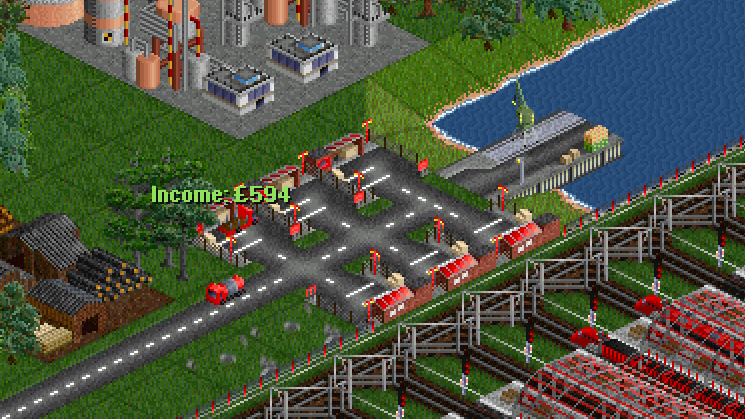
\includegraphics[width=\columnwidth]{assets/openttd-screenshot.png}
\caption{A small section of an OpenTTD (version 12.2) game at the moment when income is received for delivering goods by road. Also shown is part of a railway network, a port for ships, an oil refinery, and a sawmill.}
\label{fig:openttd}
\end{figure}


OpenTTD was created as a game for recreation. However, it is remarkably flexible: it has been successfully used as a tool to research artificial intelligence (AI) and machine learning (ML) algorithms \cite{wisniewski2011artificial, rios2009trains, bijlsma2014evolving}, scalability and mobile applications \cite{jiang2018mirroring}, and as a teaching aid \cite{HansenMuprhie2018}. It allows a single player to play in a non competitive world building mode, multiple human players playing cooperatively or competitively, and allows so-called custom AI-players that each control a company via code not part of the OpenTTD, but part of extensions to it written in the Squirrel language.

Using OpenTTD as a tool for research is the focus of this project, and specifically the focus is the development of a tool that augments its existing features for repeatable, replicable, \& reproducible research.

\section{A brief history of learning from simulation games}

Games have a long history of being used as tools beyond recreation, and specifically as tools to simulate the real world in order to take conclusions about the game environment and apply them to the world outside of the game, with war games doing this as far back even to ancient periods \cite{mayer2009gaming}. One of the world's oldest board game, Go (the `game of encircling territories' to literally translate its Mandarin name), originating in China approximately 4000 years ago and popular since, has been argued to embody strategies that bear a striking resemblance to Chinese strategies of war and diplomacy, and these arguments have been paired with suggestions that Americans could better understand current (as of 2004) real-world Chinese strategies by learning Go \cite{lai2004learning}. Go is played on a grid, much like OpenTTD, suggesting also that OpenTTD's discretized simplification of space also has a long history in simulation.

The military-style/war games eventually evolved to logistic simulations, albeit still in military context. Fore example based MONOPOLOGS \cite{jackson1959learning} that is often credited as the first computerised logistics simulation game - SAY WHEN AND WHAT USED FOR. Then the MIT beer game - to illustrate something in supply chains. These then evolved to games that informed policy making - EXAMPLE.


This evolved [REF]

----

OpenTTD is part of a wider class of games: simulation games. Simulation games have been frequently used in various fields to explore scenarios in an effort to inform policies. PUT IN LIST.

Attention is usually paid to how realistic these games are. For example, \cite{raghothama2013review} summarises how well a number of games, including OpenTTD, how well the games model the real world. It's worth noting that while the economic model of OpenTTD is not realistic, \cite{raghothama2013review} classes some aspects of the transportation model as realistic, albeit without justification.



\section{Repeatability, Replicatability, \& Reproducibility}



The terms repeatability, replicability, and reproducibility unfortunately do not historically have universally agreed meanings \cite{plesser_reproducibility_2018}. To add to the confusion, the ACM have swapped their definitions reproducibility and replicability \cite{association_for_computing_machiner_new_2020}. For the avoidance of doubt, I use the ACM's definitions that are current as of October 2023 \cite{association_for_computing_machiner_artifact_2020}. For some results of an experiment conducted by a team of authors, where some computer-based artefacts were created to conduct these, these can be summarised as

\begin{description}
\item[Repeatability] The authors can obtain the results again, using the same artefacts.
\item[Reproducibility] A different team can obtain the results, using the original authors' artefacts.
\item[Replicability] A different team can obtain the results, without using any of the original authors' artefacts.
\end{description}

The strongest of these these, replicability, does not require a full re-implementation of all artifacts used in the research, but only those created by the original team. In OpenTTD terms, if an author writes a custom AI that is used in experiments, only that AI would need to be implemented by another team to replicate the research. OpenTTD itself would not need to be re-implemented in order for experiments to satisfy the definition of replicability.

Beyond just supplying definitions, the ACM also provide a system of 5 badges, as seen in Figure \ref{fig:acm_badges}. These can be applied to published research to incentivise research authors to make it so their research is reproducible and replicable by other teams. Other similar systems of badges are available.

\begin{figure}
     \centering
     \begin{subfigure}[t]{0.3\columnwidth}
         \centering
         
\includegraphics[width=\textwidth]{assets/artifacts_available.jpg}
         \caption{Artifacts available}
         \label{fig:y equals x}
     \end{subfigure}
     \hfill
     \begin{subfigure}[t]{0.3\columnwidth}
         \centering
         
\includegraphics[width=\textwidth]{assets/artifacts_evaluated_functional.jpg}
         \caption{Artifacts evaluated functional}
         \label{fig:three sin x}
     \end{subfigure}
     \hfill
     \begin{subfigure}[t]{0.3\columnwidth}
         \centering
         
\includegraphics[width=\textwidth]{assets/artifacts_evaluated_reusable.jpg}
         \caption{Artifacts evaluated reusable}
         \label{fig:five over x}
     \end{subfigure}
    \par\bigskip
     \begin{subfigure}[t]{0.3\columnwidth}
         \centering
         
\includegraphics[width=\textwidth]{assets/results_reproduced.jpg}
         \caption{Results reproduced}
         \label{fig:five over x}
     \end{subfigure}
     \begin{subfigure}[t]{0.3\columnwidth}
         \centering
         
\includegraphics[width=\textwidth]{assets/results_replicated.jpg}
         \caption{Results replicated  safd }
         \label{fig:five over x}
     \end{subfigure}
        \caption{The ACM system of badges for reproducble research}
        \label{fig:acm_badges}
\end{figure}

It is my hope that the framework presented here will make it more likely that research using OpenTTD will be not only repeatable, reproducible and replicable, but also more likely that upon publication, given all of these badges. 

\section{Barriers to Repeatability, Replicatability, \& Reproducibility}

\section{Review of research using OpenTTD}

Note - put this after the 3Rs stuff. The 3Rs stuff will have (especially for reproduciliby and replicability) barriers, and so I should be able to basically discuss the research, stating what barriers it seems to have.

\begin{itemize}
\begin{item}
Some papers list how they found all their upstream papers, in a light meta-analysis way. Worth it here? If I'm arguing something is lacking in particular, then maybe yes, because I sort of need evidence of an exhaustive search
\end{item}
\begin{item} Maybe this section could be split into using using OpenTTD in experiments, and just mentioning it
\end{item}
\begin{item}
\cite{fenjiro2018deep} - Mentions OpenTTD uses Deep Learning, but not partcular context or explanation. It doesn't really?? Do even any of the published AIs??
\end{item}
\end{itemize}

TODO: If we have the more structured / formal reproducibility stuff earlier, we can more properly judge the existing research.

From the found published research using OpenTTD, in my opinion there is yet to be a single case that couldn't offer significant improvements in at least one of its repeatability, replicability or replicability.

\subsection{Repeatability}

Repeatability should be the easiest of the 3Rs to achieve, especially with computer based simulation. However, much of the existing research using OpenTTD uses a low number of repeated experiments, with little or no statistical analysis, suggesting that it was not straightforward. The experiments of \cite{wisniewski2011artificial} were run just 3 times for example. The experiments in \cite{rios2009trains} were run 14 times, but not even for the same amount of in-game time.

\subsection{Reproducibility}

For reproducibility the author-supplied artifacts must be clear and available. There were references to modified OpenTTD in \cite{wisniewski2011artificial}, but the modified versions does not seem to be available. Potentially the authors could be contacted to supply their own artefacts, but this is not ideal, nor offers a strong guarantee that the artefacts supplied were exactly as they were that generated the results.

Also, the version of OpenTTD is not mentioned

The seeds of each experiements were also not supplied.

\subsection{Replicability}

This is the most difficult to judge without actually attempting to do it, and it is what.

However, if an experiment isn't even reproducible, it is even more difficult to replicate it.

\chapter{OpenTTD: its model and abilities}

A game of OpenTTD is made up of a rectangular world with one or more companies in it, typically working in competition against each other. A company is paid for transporting goods and passengers between certain combinations of industries and towns, and in order to do so it needs to invest in road, rail, sea or air infrastructure and vehicles.

Usually when using OpenTTD for recreation there would be one or more human players that each control a company. However, this is not a requirement: OpenTTD allows non-human players, so-called AI players, fully controlled by custom code supplied by the player/researcher. If there are no human players, OpenTTD also then runs deterministically - using a seed value on startup that controls all pseudo-random behavior of the game. These abilities are the core abilities that allows OpenTTD to be used in repeatable, reproducible and, hopefully, replicable simulations.

This chapter explores this model and these abilities in more detail, as well other related existing features that allow OpenTTD to be controlled programatically and ultimately used, through the OpenTTDLab framework presented in the next chapter, to run simulations. This chapter also shows that the environment of OpenTTD is a rich one; while there are clearly some unrealistic aspects, it is at least a tempting target for running simulations that could be used to extract some insights applicable to the real world.

Unless otherwise stated, the details here are from OpenTTD Wiki \cite{OpenTTDWiki}, the OpenTTD source code \cite{OpenTTDSource}, the OpenGFX source code \cite{OpenGFXSource}, the OpenTTD AI API documentation \cite{OpenTTDAIAPIDocs}, the OpenTTD GameScript API documentation \cite{OpenTTDGSAPIDocs}, or by playing OpenTTD itself. Details are correct as of OpenTTD 13.4.

\section{Field of play/simulation}

OpenTTD runs on two-dimensional rectangular tiled grid representing an area of land and sea, with some limited three-dimensional aspects. The grid size is configurable on startup between 64x64 and 4096x4096 tiles. Each tile is square, albeit presented to the user in a dimetric view; sometimes inaccurately referred to as an isometric view. Each tile does not necessarily have a single object on it, some objects can co-exist with each other depending on the object type. The positions of vehicles that carry goods and passengers, which are the main mechanism for making money in the game, are even more granular - they move and take positions at what appear to be any position on their path between destinations.

There is some concept of height - each section of a grid can have one of X possible height levels in the game, with sloping land between each level. This impacts the game in more than just a visual way: when going uphill road and rail vehicles slow down - the amount depending on the type of the vehicle, and how laden they are with goods. As discussed later, the amount they slow can have an impact on money made. Rail and road tunnels can be built by the companies, which can avoid this, but they have their downsides: they typically cost the company more to build, depending on their type have their own speed restrictions, and they can have no bends, or go up or down in terms of their height - entry and exit must be on the same level.

An example field of play, also showing some of the interface that players use to interact with the field of play is show in Figure \ref{figure:openttd-field-of-play}.

\begin{figure}[h]
\centering
\includegraphics[width=\textheight,height=\textwidth,keepaspectratio,angle=90]{assets/openttd-field-of-play.png}
\caption{A the interface of OpenTTD 13.4, showing an portion of an example transport network linking industries and towns.}
\label{figure:openttd-field-of-play}
\end{figure}

\section{Startup}

On startup of a new game/simulation, there are two classes of startup. A pre-defined scenario can be started, where the map is pre-defined, or a pseudo-random world is generated. In the pseudo-random case, the world is deterministically generated based on a seed value, and the configuration of the game. Specifically, the land, height, trees, coastlines and sea, the sizes and positions of town, and the positions and types of industries are all pseudo-randomly generated. This determinism helps OpenTTD be used for repeatable experiments.

Note that other than roads within towns, no transport infrastructure exists. It is the role of the player to build this.

\section{Agents and ticks}

OpenTTD is an agent-based system, with agents: buses, trains, planes, ships, industries and even buildings in towns to an extent running apparently independently and in accelerated real time. However, the real-time aspect is somewhat of an illusion. OpenTTD runs on the concept of \emph{ticks}, where there are 74 ticks per in-game day. During a tick, game time progresses in a deterministic way - vehicles move a certain amount, pick up or drop off a certain amount of passengers or goods, industries produce a certain amount of goods, a number of passengers are "produced" by towns wanting to travel.

This determinism makes OpenTTD particularly suitable for exactly repeatable simulations. If, for example, instead of ticks, threads were used for the various agents, since thread scheduling is in general non deterministic, then exactly repeatable experiments would not be possible.

\section{Economic model and supply chains}

The companies in OpenTTD receive money for transporting cargo and passengers between sources and destinations. The amount of money is dependant on a number of factors: the amount of cargo, the cargo type, the time taken - a shorter time results in more money - and the distance taken - a longer distance results in more money.

Industries each produce and accept certain types of cargo, depending on their industry. For example, a steel mill accepts iron ore, and produces steel. A factory accepts steel, and produces goods. The range of industries depends on the \emph{climate} that the game is started in: temperate, sub-arctic, tropical and toyland. In the temperate climate, the default, there are 12 possible industries, plus towns, which produce and accept a total of 12 types of cargo, including passengers and mail. How much each industry or town depends on on how much input cargo it has received, a hidden property of its total (pseudo-randomly chosen in pseudo-randomly generated worlds), which can also change during the game similarly pseudo randomly. The full supply chain of the temperate climate can be seen in Figure \ref{figure:temperate-supply-chains}.

Informally, there are a number immediate absurdities to the economic model. For example, as long as an industry's type can accept that type of cargo, it can accept any amount of that cargo type - for which the company that transported it receives money. This includes passengers: for example when a passenger arrives as a bus station, that particular passenger has no particular destination in mind in the game - the company will receive money for taking them anyway, but more money if they are taken further. In a similar vein, there is nothing more granular than a type of cargo: factories and oil refineries both produce so-called \emph{goods} which are accepted by all towns.

It is beyond the scope of this project to more rigorously analyse the economic model of OpenTTD, and to so work out how much any insights generated by OpenTTD simulations can be applied to the real world. It has been suggested that while the economic model is not realistic, the network effects of OpenTTD are somewhat realistic \cite{raghothama2013review} - it is the aim of this project that the OpenTTDLab framework presented in the next chapter offers a mechanism to better study these.

\begin{figure}[h]
\centering
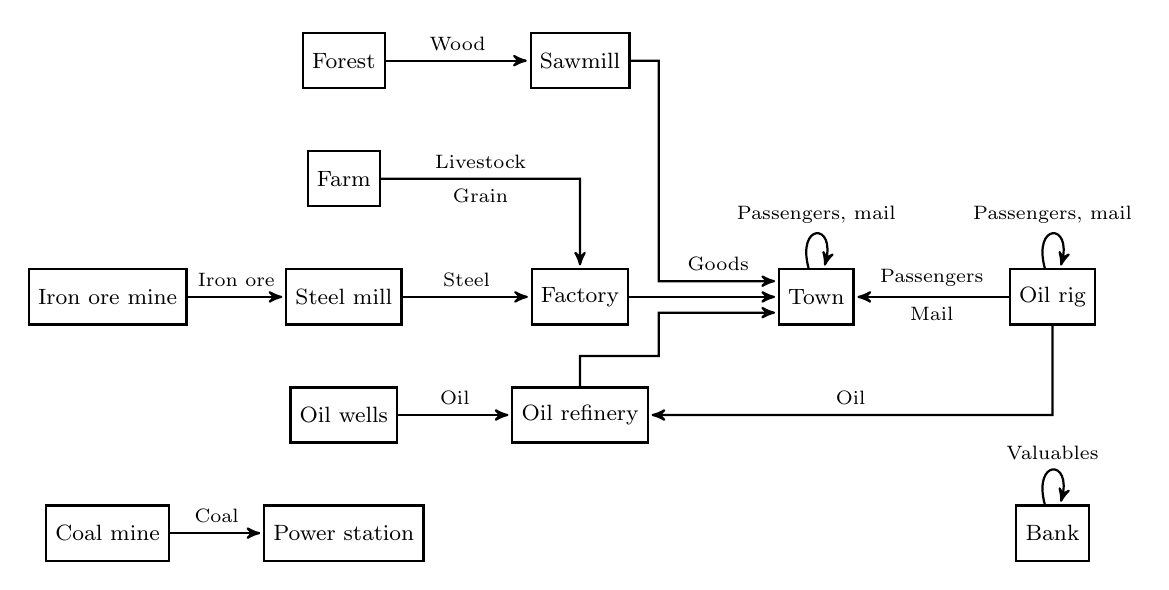
\begin{tikzpicture}[->,>=stealth',shorten >=1pt,auto,node distance=3cm,thick,main node/.style={rectangle,draw}]

    \node[main node, align=center,minimum size=0.7cm] (factory) {\footnotesize Factory};
    \node[main node, align=center,minimum size=0.7cm,on grid,right=3cm of factory] (town) {\footnotesize Town};
    \node[main node, align=center,minimum size=0.7cm,on grid,right=3cm of town] (oil-rig) {\footnotesize Oil rig};
    \node[main node, align=center,minimum size=0.7cm,on grid,left=3cm of factory] (steel-mill) {\footnotesize Steel mill};
    \node[main node, align=center,minimum size=0.7cm,on grid,left=3cm of steel-mill] (iron-ore-mine) {\footnotesize Iron ore mine};
    \node[main node, align=center,minimum size=0.7cm,on grid,below=1.5cm of steel-mill] (oil-wells) {\footnotesize Oil wells};
    \node[main node, align=center,minimum size=0.7cm,on grid,above=1.5cm of steel-mill] (farm) {\footnotesize Farm};
    \node[main node, align=center,minimum size=0.7cm,on grid,above=1.5cm of farm] (forest) {\footnotesize Forest};
    \node[main node, align=center,minimum size=0.7cm,on grid,below=3cm of oil-rig] (bank) {\footnotesize Bank};
    \node[main node, align=center,minimum size=0.7cm,on grid,below=1.5cm of oil-wells] (power-station) {\footnotesize Power station};
    \node[main node, align=center,minimum size=0.7cm,on grid,left=3cm of power-station] (coal-mine) {\footnotesize Coal mine};
    \node[main node, align=center,minimum size=0.7cm,on grid,right=3cm of forest] (sawmill) {\footnotesize Sawmill};
    \node[main node, align=center,minimum size=0.7cm,on grid,below=1.5cm of factory] (oil-refinery) {\footnotesize Oil refinery};

    \path[every node/.style={font=\scriptsize}]
        (forest) edge[] node[] {Wood} (sawmill)
        (bank) edge [loop above, distance=0.6cm] node[] {Valuables} (bank)
        (coal-mine) edge[] node[] {Coal} (power-station)
        (iron-ore-mine) edge[] node[] {Iron ore} (steel-mill)
        (oil-wells) edge[] node[] {Oil} (oil-refinery)
        (oil-rig) edge[loop above, distance=0.6cm] node[] {Passengers, mail} (oil-rig)
        (factory) edge[] node[] {} (town)
        (steel-mill) edge[] node[] {Steel} (factory)
        (town) edge[loop above, distance=0.6cm] node[] {Passengers, mail} (town);

    \path[draw,->] 
    (oil-rig.south)
    -- ($ (oil-rig.center) - (0,1.5) $)
    -- node[above] {\scriptsize Oil}
    (oil-refinery.east);

    \path[draw,->] 
    (oil-rig.west)
    -- node[above] {\scriptsize Passengers} node[below] {\scriptsize Mail} 
    (town.east);

    \path[draw,->] 
    (farm.east)
    -- node[above] {\scriptsize Livestock} node[below] {\scriptsize Grain} ($ (farm.center) + (3,0) $)
    --
    (factory.north);

   \path[draw,->] 
    (oil-refinery.north)
    -- ($ (oil-refinery.center) + (0,0.75) $)
    -- ++(1,0)
    -- ++(0,0.55)
    -- ($ (town.west) - (0,0.2) $);

    \path[draw,->] 
    (sawmill.east)
    -- ($ (sawmill.center) + (1,0) $)
    -- ++(0,-2.8)
    -- node[above] {\scriptsize Goods} ($ (town.west) + (0,0.2) $);

\end{tikzpicture}
\caption{The possible supply chains of the temperate climate of OpenTTD 13.4, showing what types of cargo industries and towns accept and produce. Adapted from \cite{TemperateFlowChart}.}
\label{figure:temperate-supply-chains}
\end{figure}

\section{The possible actions a player can take}

\section{Algorithm of each player}

\section{Algorithm of the game}



List the goods!

\begin{itemize}
\begin{item}Industries produce a certain amount of goods per tick based on a "how good" they are, combined with a pseudo-random varience\end{item}
\begin{item}Industries will accept any amount of the range of goods they accept, and pay\end{item}
\begin{item}The amount of money the industries pay increases with the distance they travelled according to a fixed formula for each good type\end{item}
\begin{item}The amount of money the industries pay decreases with the amount of time it took\end{item}
\end{itemize}

For the purpose of the above, industries include towns, which produce passengers and mail.

It is beyond the scope of this project to analyse this model in any formal way, and to work out exactly how results gleamed by using OpenTTD can be applied to the real world.

\section{Transportation and station types}

\section{OpenTTD AIs}

OpenTTD AIs are scripts that can be plugged into OpenTTD at runtime that allows it to control a company. It has a rich API, with approximately X functions in total.

It work within "tick" framework - every tick of the game a certain amount of the script can progress.

This is the core feature that allows OpenTTD to be used to experiment how different strategies of AIs affect the outcome, and so, to an extent, simulate properties of the real world.

\section{Configurability}

There are a number of configuration - it's not useful to list them all. However, there are 

OpenTTD as of version 13.4 has over X command line options and Y configuration options that allow the player to customise how it behaves when playing - it is not useful to review them all here. However the ones that are particularly applicable to a for repeatable, reproducible, and replicable research, and leveraged by OpenTTDLab are below

\begin{itemize}
\begin{item}
OpenTTD accepts a random seed as input. This is used to then generate the initial world in a deterministic way, and then also affect any other pseudo-random behaviour. If there is no user input duing the game, which is the case if only playing with AIs, this makes the entire game deterministic based on the input
\end{item}
\begin{item}
OpenTTD does not have an end
\end{item}
\begin{item}
Autosave
\end{item}
\begin{item}
Startup script to immedaitely load AIs 
\end{item}
\end{itemize}


\section{OpenGFX}

It's somewhat of a misnomer - it's not just graphics but details of vehicles, which affect gameplay, and the simulation. It's important to have the exact version

\section{The save game format}

OpenTTD saves its data in a custom binary format - its so-called savegame format. OpenTTD offers an extremely basic tool for extracting some data from this format. However, a separate Python based tool is available to extract data from save games

\section{What doesn't exist}

\begin{itemize}
\begin{item}
With reference to the the desired things from the reproducibility section, mention things that don't exist
\end{item}
\end{itemize}

Running many experiments. Extracting data for analysis.

\chapter{The framework}

\begin{figure}[h]
\centering
\includesvg{assets/openttdlab-logo.svg}
\caption{The OpenTTDLab logo. I created this based on the existing GPLv2-licensed OpenTTDLogo, and it is displayed alongside the code of OpenTTDLab in its public documentation.}
\label{fig:openttlab-logo}
\end{figure}

As discussed in Chapter 1, repeatability is in the domain of the original researchers, while both replicability and reproducibility are in the domain of other researchers armed with the original results. Given the different aims and audiences, it's not immediate that a single tool can be used in all of these. However, the Python framework OpenTTDLab I created attempts to be useful in all of these: to augment the existing behaviour of OpenTTD of Chapter 2 to help address at least some of the barriers detailed in Chapter 1. This chapter details the design process I followed to create OpenTTDLab to do this, and the resulting internal behaviour and user-facing features of the framework.

\section{Design and creation process}

A lightweight and highly agile process was used to design and create OpenTTDLab, the high level features of which are shown figure \ref{fig:solo-agile}. After the problems to solve have were identified, as discussed in Chapter 1, there were many cycles of writing usage documentation for code, writing code, and using the code, either to construct the results of Chapter 4 or in tests; and each of these with tight cycles of evaluating the outputs of these activities and informally judging if the code does (or would if it existed) help produce research that was repeatable, replicable and reproducible. Each of these activities would inform each other in tight cycles.

\begin{figure}[h]
\centering
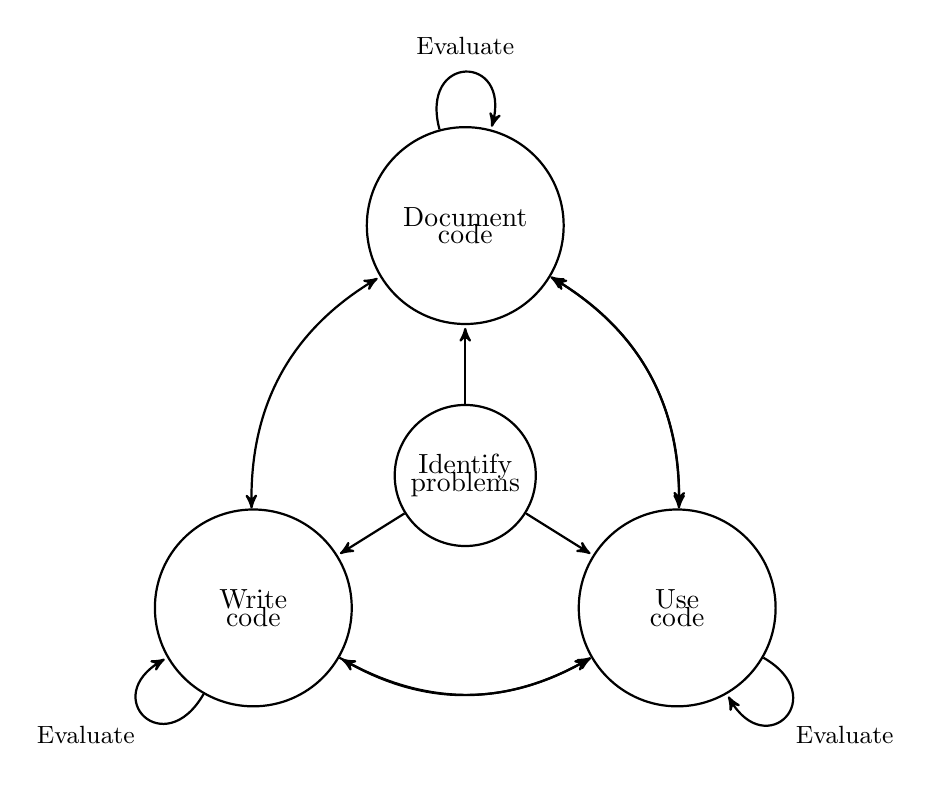
\begin{tikzpicture}[->,>=stealth',shorten >=1pt,auto,node distance=3cm,
                    thick,main node/.style={circle,draw}]

    % https://tex.stackexchange.com/a/102266
    \tikzset{
        position/.style args={#1:#2 from #3}{
            at=(#3.#1), anchor=#1+180, shift=(#1:#2)
        }
    }

    \node[main node, align=center] (reqs) {Identify\\[-2mm]problems};
    \node[main node, align=center,minimum size=2.5cm] (code) [position=90:1cm from reqs] {Document\\[-2mm]code};
    \node[main node, align=center,minimum size=2.5cm] (docs) [position=-148:1cm from reqs] {Write\\[-2mm]code};
    \node[main node, align=center,minimum size=2.5cm] (expe) [position=-32:1cm from reqs] {Use\\[-2mm]code};

    \path[every node/.style={font=\small}]
        (reqs) edge [] node[] {} (code)
               edge [] node[] {} (expe)
               edge [] node[] {} (docs)
        (docs) edge [in=-150,out=-120,distance=1cm,loop] node[] {Evaluate} (docs)
               edge [bend left,arrows=<->] node[] {} (code)
               edge [bend right] node[left] {} (expe)
        (code) edge [distance=1cm,loop above] node[yshift=0.1cm] {Evaluate} (code)
               edge [bend left,arrows=<->] node[] {} (expe)
        (expe) edge [in=-60,out=-30,distance=1cm,loop] node {Evaluate} (expe)
               edge [bend left,arrows=<->] node[] {} (docs)
               edge [bend right,arrows=<->] node[] {} (code);
\end{tikzpicture}
\caption{The process I followed designing and creating OpenTTDLab. After identifying the problems that I'm trying to address, I conducted cycles of documenting code (that may not have existed), writing the code, and using the code, all coupled with tight cycles of evaluating how it solved, or would solve, the problem of running experiments using OpenTTD that were repeatable, replicable and reproducible.}
\label{fig:solo-agile}
\end{figure}

I use the term lightweight in that there were no \emph{events} that are common to \emph{Scrum}-like processes \cite{SCRUM} (often known as \emph{ceremonies} from my own experience), and with one exception, no phases planned in advance as is prescribed, for example, for UK government services \cite{GOVUKAgile}. And I describe the process as highly agile because in some cases iterations would take literally seconds, especially when writing documentation.

This was in fact the one exception to not having phases planned in advance: I did plan to create an initial version of light usage documentation very early in the project. Taking inspiration from Tom Preseton Warner's Readme driven development \cite{ReadmeDrivenDevelopment} and Amazon's Working Backwards method \cite{bryar2021working}, both at the beginning and throughout the project I would usually write such documentation for code without the code first existing. This allowed me to imagine it being used, evaluate how well it would solve the problems I'm trying to solve, and change its design accordingly by quickly changing its documentation. Of course, documentation for code that does not exist has very little value, so I moved quickly to writing and using code, mostly informed by "Working software is the primary measure of progress" and "Deliver working software frequently" from the Agile Manifesto \cite{beck2001manifesto}, which I judge to be the most useful parts of the Agile Manifesto, especially when working alone (albeit with advice from others) when the other parts are less applicable - they focus on communication between different people involved in project.

I did not attempt to keep a precise record of the cycles. However, as a guide, the GitHub repository that stores the history of code changes can be used. I created 72 releases, which I labelled v0.0.1 through v0.0.72, 215 pull requests (PRs), and over 250 non-merge commits in the repository, and each of these I evaluated against problems and desired properties of Chapter 1, and then carried on with more of the same activity, or another activity of Figure \ref{fig:solo-agile}.

The first version, v0.0.1, was the result of a fork from Patric Stout's \emph{OpenTTD-savegame-reader} \cite{Stout2024}, an existing project that extracts data from OpenTTD save game files - files that save the state of play in OpenTTD that allows players to exit but resume at the same point later. This could be used when using OpenTTD to run simulations, albeit in a time consuming way because the manual steps involved.

Then, but still from very early in the process, v0.0.3, I created and maintained a small suite of tests for OpenTTDLab, asserting on its high level behaviour. The tests were not just for asserting on the behaviour of the code, they were also a special case of "Use code" in the design process: they allowed me to extremely quickly gauge the suitability of the design of the OpenTTDLab, because to write test tests I had to use OpenTTDLab in a way very similar to those that experimenters would have to use it.

This leads to the main downside of this process. While the process allowed a high number of cycles of evaluations, all feedback and evaluation is from myself, from either running the code or, even worse, just imagining running the code. Being the designer I know it extremely well and so am ill-placed to evaluate what amounts to its ease of use for people that don't know it as well: I'm essentially \emph{marking my own homework}, and in some cases before it was even written. User research was not included in the process in order to limit the scope of the project, and to allow as many iterations as possible within the available time, which includes using the framework to produce the results of Chapter 4 (and the scaling results of Chapter 3).

The other downside is that the process optimizes for the specific usage I chose, which as will be seen in Chapter 4, are repeating experiments, rather than reproducing or replicating them. However, as discussed in Chapter 1, repeating experiments is part of reproducing and replicating them, and so focusing on repeating experiments is a suitable way of limiting the scope of the project while still producing behaviour that should be a useful component when reproducing or replicating them.


\section{High level architecture}

Through the design and creation process, particularly after evaluation, I made a number of high level architectural decisions: the use of Python, behaving identically where possible on different platforms, automatically downloading OpenTTD and OpenGFX, supporting both AIs in the local filesystem, and automatically downloading AIs, caching, and the use of parallelisation.

I chose Python as the main language for both the internals of OpenTTDLab and its user-facing interface. I knew Python well, a savegame parser for OpenTTD was available in Python \cite{Stout2024} that the project forked from, programs written in Python are mostly platform independant, and anecdotally it's a popular language in data science and data analysis. To make sure OpenTTDLab did not depend on specific behaviour of a single Python version, which could impede repeatability and replicability of experiments, I made sure that the tests I wrote ran on multiple versions of Python.

OpenTTDLab automatically downloads OpenTTD, OpenGFx, and AIs. This was a direct consequence of running 

It also supports using AIs on the local filesystem. When replicating experiments that use AIs, when the experimenters do not directly use the code of the original researchers, I suspect a fast feedback is needed when writing code and running experiments using that code. While downloading AIs supports replicating experiments using published AI code, reproducing experiments would not us the AI code, and would use code on the local file system.

On the request of one of the maintainers of OpenTTD, OpenTTDLab caches OpenTTD, OpenGFX, and the AIs that it downloads....

I know from experience that there can be problems when a program written on one platform is used on another. While Python is meant to be platform independent, and OpenTTD runs on Linux, Windows and macOS, I discovered that not only are the OpenTTD binaries different for each platform, but also the processes of downloading, installing, and starting OpenTTD are different. So I made sure that OpenTTDLab detects the platform, and performs the appropriate steps for that platform, without the experimenter being concerned, so any Python code using OpenTTDLab written on one platform should run on another unchanged and behave identically. The tests run identically on each of these platforms, and so gives evidence of this property of OpenTTDLab.

From running OpenTTDLab, and being frustrated by run times, I decided to make OpenTTDLab run its experiments in parallel, by running multiple threads, and from each of these threads triggering OpenTTD configured appropriately for that experiment. The scaling results of these are shown in Section ...

\section{API design}

??

\section{Rejected features}

I considered a number of features while creating OpenTTD - due to the high number of cycles of the design process, there are too many to recall or recount. However, there are three that I think are particularly relevant.

Firstly was the saving of results of experiments to a file, rather than to an ephemeral data structure in memory. If done well, I suspected this would have been a valuable feature: it could have aided analysis, made it easier to... . However.... SQLite, the most popular database in the world REF, also recommended by the US Library of Congress, would be an obvious candidate. But even after this choice, how to convert OpenTTDLab's arbitrary nested file structure into a relational model to be stored in a SQLite file is not obvious. Due to the relative permanency of any choice, in that once created, the files should be able to be interpreted in the long term, this should be done after examples of OpenTTDLab have been created.

Secondly, I considered some sort "verification" step built into the API - starting with v0.0.2 and removed in XXX, with at the time a vague notion of it being used in reproducing or replicating experiments. However, I found even the skeleton of this made generating the results of Chapter 4 awkward, or in more formal terms it and it seemed so far removed from what I knew of similar APIs.

Finally, I considered a file format for the configuration. This was rejected for essentially a combination of the previous two reasons - any file format must be carefully designed, and it seemed to make things awkward rather than easier.

Custom build of OpenTTD?? Local file?

Versions of these features could well be added in future versions, but ideally in a way that does not make repeating experiments such as those in Chapter 4 significantly more awkward and so negatively affecting the repeatabilty of experiments using OpenTTDLab, and so, given that repeating experiments is part of reproducing and replicating them, in a way that also doesn't make these activities more difficult.

Tidy results?

\section{Screenshots}

... saves screenshots! Mostly just for me



\section{Algorithm}

\begin{algorithm}
\caption{The core algorithm of OpenTTDLab}\label{alg:three}
\KwData{The list of experiments to run, where each is defined by the seed, number of days, list of AIs and parameters to pass to the AIs. Versions of OpenTTD and OpenGFX}
\KwResult{The parsed save games from every month of game time for every experiment} 
 fetch everything that needs to be fetched (not stuff that is already in cache...)\;
 setup threaded pool for workers\;
 \ForEach(in parallel up to {max\_workers}){experiment in experiments}{
  run experiment by running OpenTTD\;
  parsing all the save games\;
 }
\end{algorithm}

\section{Scaling}

I conducted a brief investigation into how well OpenTTDLab scales with the number of worker processes by running the same set of 50 simulations, but distributing the work between 1 to 8 worker processes, and seeing how the runtime changes. I also did these tests when passing the full set of results back to the controlling process, and for only passing a minimal amount of data: the date, the company value at that date, and if an error occurred. All the simulations were conducted on a 2020 Apple M1 with 8 CPU cores, 16GB of RAM, OpenTTDLab 0.0.72, OpenTTD 13.4, Python 3.11.0, trAIns 2.1 retrieved from the BaNaNaS content service with MD5 hash of c4c069dc797674e545411b59867ad0c2, and running for seeds 0 to 49, and each for a total of 1465 in-game days (just over 4 in-game years). The Python code to run the experiments can be seen in Appendix \ref{chapter:scaling-running-code}, and the code to subsequently process and visualise the results in Appendix \ref{chapter:scaling-analyis-code}.

\begin{figure}[h]
\centering
\begin{gnuplot}[terminal=cairolatex,terminaloptions={size 5,3}]
set datafile separator ","
set style fill pattern 2
set key left top
set key invert
set grid ytics
set ylabel 'Time (seconds)'
set yrange [0:]
set xlabel 'Number of worker processes'
plot 'notebooks/01_scaling_results_02_wallclock_times.csv' \ 
   using 1:2 with linespoints ls 1 title 'All data', \
   '' using 1:3 with linespoints ls 2 title 'Minimal data'
\end{gnuplot}
\caption{Total wallclock time of when running 50 experiments using OpenTTDLab between 1 and 8 worker processes, comparing returning all data to the controlling process, and returning a minimal amount of data. Using more worker processes results in a shorter runtime: for example using 8 worker processes uses about 20\% of the runtime as using 1 worker process. Returning a minimal amount of data also results in shorter runtime: approximately 30\% faster for each number of processes in the experiment.}
\label{figure:scaling-wallclock-time}
\end{figure}

As can be seen from Figure \ref{figure:scaling-wallclock-time}, wallclock time decreases as the number of processors increases, and so there is some useful parallelisation: running with 8 worker processes results in an 80\% reduction of runtime compared to running on 1 process. Also returning a minimal set of data from the worker resulted in an approximately 30\% reduction in time. One can conclude that it's worth running them on multiple workers, and to reduce the amount of data returned from the workers, especially if running a high number of experiments.

However, Figure \ref{figure:scaling-wallclock-time} also suggest that that there is an aspect of diminishing returns: for example the difference in runtime between 1 and 4 processes is much greater than the difference between 5 and 8. To better show this effect, we investigate \emph{speedup}: how many times faster the program runs for a given number of worker processes compared to the time it takes running on a single worker process. The speedup for the experiments, together with a theoretical linear speedup can be seen in Figure \ref{figure:scaling-speedup}.

\begin{figure}[h]
\centering
\begin{gnuplot}[terminal=cairolatex,terminaloptions={size 5,3}]
set datafile separator ","
set style fill pattern 2
set key left top
set key invert
set grid ytics
set ylabel 'Speedup'
set yrange [1:]
set xlabel 'Number of worker processes'
plot 'notebooks/01_scaling_results_03_speedups.csv' \ 
   using 1:4 with linespoints ls 3 title 'Linear scaling', \
   '' using 1:2 with linespoints ls 1 title 'All data', \
   '' using 1:3 with linespoints ls 2 title 'Minimal data'
\end{gnuplot}
\caption{Speedup when running 50 experiments using OpenTTDLab between 1 and 8 worker processes, comparing returning all data to the controlling process, and returning a minimal amount of data. Speedup is initially linear, but becomes worse as the number of worker processes increases, especially from 5 worker processes onwards. At 8 worker processes the speedup is approximately 4.5. The scaling profiles for both sets of experiments are almost identical. Given that wallclock time is reduced when returning less data from worker to controlling process, as can be seen in Figure \ref{figure:scaling-wallclock-time} this suggests that returning less data to the controlling process reduces both parallel and serial runtime of the code.}
\label{figure:scaling-speedup}
\end{figure}

It can be seen that up to 4 processors the scaling is just under linear, but after 4 processors the scaling is much worse. It can also be seen that the scaling profiles of returning all data and minimal data from the worker processes is almost identical.

A reason for the greater-difference-from-linear scaling when the number of processors is greater than 4 could come from that the cores are not identical. According to Apple \cite{AppleM1Overview} 4 cores are high performance, but the other 4 are lower performance (but have higher efficiency in terms of power usage). The scaling profiles found appears roughly consistent with the high/lower performance split, and suggests that the high performance cores being used in preference to the low performance cores.

Another reason for the deviation from linear speedup is Amdhal's Law that describes how speedup is related to proportion of the program that runs in serial. This law is usually formulated as

\begin{equation}
S_p = \frac{1}{(1-p) + \frac{p}{s}}
\end{equation}
%
where $S_p$ is the speedup of the entire program, $p$ is the proportion of the program that has been parallelised, and $s$ is speedup of the parallelised part of the program. The most relevant consequence of this is that $\lim_{S\to\infty} S_p = \frac{1}{1-p}$. This means that for example, even if 95\% of a program is parallelised, then the maximum speedup is $\frac{1}{1-0.95}=20$, even if thousands of processes are used.

This suggests that a way of increasing this limit is to reduce proportion of runtime in serial code. However, in light of Amdhal's law the identical scaling profiles in Figure \ref{figure:scaling-speedup} suggest that changing the amount of data returned from the worker processes does not change the overall proportion of runtime in serial code. Given wallclock time reduces with less data transferred, it's reasonable to suspect that reducing the data transferred reduces parallel and serial runtimes in the same proportions, possibly from the serialisation and deserialisation involved. Thus removing all data transfer is not likely to improve scaling. Also, one way to remove all data transfer is to use threads rather than processes, but threads in Python are subject to the Global Intepreter Lock (GIL), and so in many cases increases the proportion of serial code compared to using processes, there is a strong reason to suspect that this will make scaling worse, not better.

So a reasonable next step would be to investigate what else in the program could be running serially. This is potentially not a trivial project - for example it might be from what appears to be parallel sections of the code when examining the algorithm or the Python code, but it accesses a shared resource under contention from the other processes, perhaps even indirectly. As examples, in general there some types of memory caches are shared between cores, or reading or writing to disk  may also effectively be done serially, or at least not fully parallel up to the number of cores. To understand and improve upon the current behaviour this would need a more in-depth understanding of the computer architecture being run on, and profiling of the Python code to understand where time is being spent. This is beyond the scope of the project and so is left to further work.

However the conclusions we can draw here are that OpenTTDLab can utilise multiple cores to reduce runtime of simulations, albeit imperfectly, and that even though reducing the amount of data returned from the workers does not improve scaling, it can be an effective way to reduce wallclock runtime, and so these features of OpenTTDLab are justified and should be leveraged when running experiments.

\section{Promotion}

Hmmm... is this being shoehorned in?? I guess I think it's important... can I argue that? Why is it important in terms of the 3Rs.


\chapter{Example results}

To get evidence of OpenTTD's usefulness in terms of repeatable, reproducible and replicable experiments, I used OpenTTD in 3 different situations. Firstly, to perform a more in-depth analysis of 2 existing OpenTTD AIs than seems to have been performed already, even by their authors. Secondly, to explore how a single parameter can change how a new simple AI performs, and shows that OpenTTDLab can be used to explore risk-benefit trade offs in basic supply chains. And finally to show how OpenTTDLab can be used to programmatically optimize this parameter using a basic algorithm.

\section{Replicating results}
\lstset{numbers=left,frame=tb,basicstyle=\linespread{0.7}\ttfamily\footnotesize}
\lstinputlisting[language=Python,float,caption=A floating example]{assets/replicating_results_core.py}

\section{Simple parameterised OpenTTD AI}

From the previous section, OpenTTDLab makes it straightforward to compare existing AIs, and its richness of output allows informed speculation as to the reasons for their behaviour differences. However, this doesn't by itself allow for a more detailed analysis of the behaviour of supply chains. OpenTTDLab's feature of running experiments over a range of configuration parameters passed to an AI allows for this.

So I constructed a simple parameterised AI. At runtime, the AI chooses the 2 largest towns, find a route between them, builds a road over this route, a depot and station at each end, and builds a configurable number of buses that carry between the two stations. The algorithm in more detail can be seen in Algorithm \ref{algorithm:simpleai}, with the core Squirrel code of the AI in Appendix X, with the Python code to run the experiments in Appendix Y.

The number of buses varied between 1 and 16, and each run was for 50 years, with 50 runs for each configuration covering random number generator seeds between and 1 and 50 inclusive.

\subsection{Results}

As can be seen in Figure XX, by the end of the 50 years, there appears to be a clear winner - on average the runs with 16 buses have more money in the bank than the others. It can be seen that early in the game, on average the configurations with 16 buses had the lowest amount of money, suggesting that in this very simplified situation, and with the caveat that the economic model of OpenTTD has been argued to be unrealistic REF, it seems to be the case that \emph{you have to spend money to make money}.

However, the situation is more complex. When taking into account the distributions, for example in, it's clear that while on average 16 buses are better, there is also greater risk with 16 buses than with the one - there is a higher chance of losing more money than with a single bus.

There is also an interesting convergence point around 1978: all configurations on average have on average the same amount of money in the bank. At the moment the reason for this convergence point is so far unexplained. As can be seen in Figure X, this convergence it is certainly not true that every run of the game makes the same amount of money - the distributions of money for 1 and 16 buses remains wide.

\begin{algorithm}
\caption{Simple parameterised OpenTTD AI}\label{alg:three}
\KwData {Seed, the number of buses to build in the AI N}
 (OpenTTD generates the map deterministingly based on the seed) \;
 Fetch list of towns \;
 Sort list of towns \;
 Choose 2 biggest \;
 \While{not found route}{
  Continue to find route \;
 }
  \ForEach{step in route}{
  build step\;
 }
 build depot\;
 build station\;
 \ForEach{bus in buses}{
  build bus\;
  give orders to move between the 2 towns\;
 }
\label{algorithm:simpleai}
\caption{Test}
\end{algorithm}

\begin{figure}[h]
\centering
\begin{gnuplot}[terminal=cairolatex,terminaloptions={size 5,3}]
set datafile separator ","
set style fill pattern 2
set key left top
set key invert
set grid ytics
set format y "%.0s%c"
set xtics 3600*24*365*5
set xdata time
set format x "%Y"
set timefmt "%Y-%m-%d"
set ylabel 'Money in the bank $\textrm{\pounds}$'
set xlabel 'Date'
set xrange ["1949-01-01":"2001-01-01"]
plot 'assets/own-buses-means-standard_deviation.csv' \ 
   using (timecolumn(1, '%Y-%m-%d')):6 skip 2 with lines title 'Mean 16 buses', \
   '' using (timecolumn(1, '%Y-%m-%d')):5 skip 2 with lines title 'Mean 8 buses', \
   '' using (timecolumn(1, '%Y-%m-%d')):4 skip 2 with lines title 'Mean 4 buses', \
   '' using (timecolumn(1, '%Y-%m-%d')):3 skip 2 with lines title 'Mean 2 buses', \
   '' using (timecolumn(1, '%Y-%m-%d')):2 skip 2 with lines title 'Mean 1 bus'
\end{gnuplot}
\caption{Money in the bank for my own simple AI: 1 vs 16 buses}
\label{fig:supplychainresiliance}
\end{figure}

\begin{figure}[h]
\centering
\begin{gnuplot}[terminal=cairolatex,terminaloptions={size 5,3}]
set datafile separator ","
set style fill pattern 2
set key left top
set key invert
set grid ytics
set format y "%.0s%c"
set xtics 3600*24*365*5
set xdata time
set format x "%Y"
set timefmt "%Y-%m-%d"
set ylabel 'Money in the bank $\textrm{\pounds}$'
set xlabel 'Date'
set xrange ["1949-01-01":"2001-01-01"]
plot 'assets/own-buses-means-standard_deviation.csv' \ 
   using (timecolumn(1, '%Y-%m-%d')):($6+$10):($6-$10) skip 2 with filledcurves lc rgb '#cccccc' title "$\\pm \\textrm{1 Standard deviation}$", \
   '' using (timecolumn(1, '%Y-%m-%d')):6 skip 2 with lines title 'Mean 16 buses', \
   '' using (timecolumn(1, '%Y-%m-%d')):($6+$10) skip 2 with lines lc rgb '#cccccc' title '', \
   '' using (timecolumn(1, '%Y-%m-%d')):($6-$10) skip 2 with lines lc rgb '#cccccc' title '', \
   '' using (timecolumn(1, '%Y-%m-%d')):($2+$6):($2-$6) skip 2 with filledcurves lc rgb '#cccccc' title "$\\pm \\textrm{1 Standard deviation}$", \
   '' using (timecolumn(1, '%Y-%m-%d')):2 skip 2 with lines title 'Mean 1 bus', \
   '' using (timecolumn(1, '%Y-%m-%d')):($2+$6) skip 2 with lines lc rgb '#cccccc' title '', \
   '' using (timecolumn(1, '%Y-%m-%d')):($2-$6) skip 2 with lines lc rgb '#cccccc' title ''
\end{gnuplot}
\caption{Money in the bank for my own simple AI: 1 vs 16 buses}
\label{fig:supplychainresiliance}
\end{figure}

% \subsection{Discussion}

% Th


\section{Programmatically optimising AI parameter}

The framework has been used to extract how the bank balance from OpenTTD change over time for a company controlled by the TrainAI as in \label{fig:value-over-time}. The 

\begin{itemize}
  \item This has been created using a non-modified version of OpenTTD 13.1.
  \item The exact random seeds are shown
  \item There are 50 experiments run
  \item Each is run for the same amount of in game time
\end{itemize}

The output of the seeds used, all settings, OpenTTD version, without modification, should make the experiments repeatable, reproducible, and ideally replicable. Thus it is an improvement in these terms over many of the results reviewed in section 4.

A limitation of the framework is that the AI version used doesn't seem to have a version.

\begin{figure}[h]
\centering
\begin{gnuplot}[terminal=cairolatex,terminaloptions={size 5,3}]
set key autotitle columnhead
set datafile separator ","
set style fill pattern 2
set key left top
set key invert
set grid ytics
set format y "%.0s%c"
set xdata time
set format x "%Y"
set timefmt "%Y-%m-%d"
set xtics 3600*24*365
set mxtics 12
set ylabel 'Money in the bank $\textrm{\pounds}$'
set xlabel 'Date'
set xrange ["1950-01-01":"1953-02-01"]
plot 'assets/trainsai-means-standard-dev.csv' \ 
   every ::::36 using (timecolumn(1, '%Y-%m-%d')):($2+$3):($2-$3) with filledcurves lc rgb '#cccccc' title "$\\pm \\textrm{1 Standard deviation}$", \
   '' every ::::36 using (timecolumn(1, '%Y-%m-%d')):2 with lines title 'Mean', \
   '' every ::::36 using (timecolumn(1, '%Y-%m-%d')):($2+$3) with lines lc rgb '#cccccc' title '', \
   '' every ::::36 using (timecolumn(1, '%Y-%m-%d')):($2-$3) with lines lc rgb '#cccccc' title ''
\end{gnuplot}
\caption{The mean of money in the bank for TrainsAI over the first 36 months}
\label{fig:supplychainresiliance}
\end{figure}

\begin{figure}[h]
\centering
\begin{gnuplot}[terminal=cairolatex,terminaloptions={size 5,3}]
set key autotitle columnhead
set datafile separator ","
set style fill pattern 2
set key left top
set key invert
set grid ytics
set format y "%.0s%c"
set xtics 3600*24*365*5
set xdata time
set format x "%Y"
set timefmt "%Y-%m-%d"
set ylabel 'Money in the bank $\textrm{\pounds}$'
set xlabel 'Date'
set xrange ["1949-01-01":"1981-01-01"]
plot 'assets/trainsai-means-standard-dev.csv' \ 
   using (timecolumn(1, '%Y-%m-%d')):($2+$3):($2-$3) with filledcurves lc rgb '#cccccc' title "$\\pm \\textrm{1 Standard deviation}$", \
   '' using (timecolumn(1, '%Y-%m-%d')):2 with lines title 'Mean', \
   '' using (timecolumn(1, '%Y-%m-%d')):($2+$3) with lines lc rgb '#cccccc' title '', \
   '' using (timecolumn(1, '%Y-%m-%d')):($2-$3) with lines lc rgb '#cccccc' title ''
\end{gnuplot}
\caption{The mean of money in the bank for TrainsAI over time over 50 experiments for 30 years}
\label{fig:supplychainresiliance}
\end{figure}

\begin{figure}[h]
\centering
\begin{gnuplot}[terminal=cairolatex,terminaloptions={size 5,3}]
set key autotitle columnhead
set datafile separator ","
set style fill pattern 2
set key left top
set key invert
set grid ytics
set format y "%.0s%c"
set xdata time
set format x "%Y"
set timefmt "%Y-%m-%d"
set xtics 3600*24*365
set mxtics 12
set ylabel 'Money in the bank $\textrm{\pounds}$'
set xlabel 'Date'
set xrange ["1950-01-01":"1954-02-01"]
plot 'assets/pathzilla-means-standard-dev.csv' \ 
   every ::::48 using (timecolumn(1, '%Y-%m-%d')):($2+$3):($2-$3) with filledcurves lc rgb '#cccccc' title "$\\pm \\textrm{1 Standard deviation}$", \
   '' every ::::48 using (timecolumn(1, '%Y-%m-%d')):2 with lines title 'Mean', \
   '' every ::::48 using (timecolumn(1, '%Y-%m-%d')):($2+$3) with lines lc rgb '#cccccc' title '', \
   '' every ::::48 using (timecolumn(1, '%Y-%m-%d')):($2-$3) with lines lc rgb '#cccccc' title ''
\end{gnuplot}
\caption{The mean of money in the bank for Pathzilla over the first 48 months}
\label{fig:supplychainresiliance}
\end{figure}

\begin{figure}[h]
\centering
\begin{gnuplot}[terminal=cairolatex,terminaloptions={size 5,3}]
set key autotitle columnhead
set datafile separator ","
set style fill pattern 2
set key left top
set key invert
set grid ytics
set format y "%.0s%c"
set xtics 3600*24*365*5
set xdata time
set format x "%Y"
set timefmt "%Y-%m-%d"
set ylabel 'Money in the bank $\textrm{\pounds}$'
set xlabel 'Date'
set xrange ["1949-01-01":"1981-01-01"]
plot 'assets/pathzilla-means-standard-dev.csv' \ 
   using (timecolumn(1, '%Y-%m-%d')):($2+$3):($2-$3) with filledcurves lc rgb '#cccccc' title "$\\pm \\textrm{1 Standard deviation}$", \
   '' using (timecolumn(1, '%Y-%m-%d')):2 with lines title 'Mean', \
   '' using (timecolumn(1, '%Y-%m-%d')):($2+$3) with lines lc rgb '#cccccc' title '', \
   '' using (timecolumn(1, '%Y-%m-%d')):($2-$3) with lines lc rgb '#cccccc' title ''
\end{gnuplot}
\caption{The mean of money in the bank for Pathzilla over time over 50 experiments for 30 years}
\label{fig:supplychainresiliance}
\end{figure}


\begin{figure}[h]
\centering
\begin{gnuplot}[terminal=cairolatex,terminaloptions={size 5,3}]
set key autotitle columnhead
set datafile separator ","
set style fill pattern 2
set key left top
set key invert
set grid ytics
set format y "%.0s%c"
set xdata time
set format x "%Y"
set timefmt "%Y-%m-%d"
set xtics 3600*24*365
set mxtics 12
set ylabel 'Money in the bank $\textrm{\pounds}$'
set xlabel 'Date'
set xrange ["1950-01-01":"1954-02-01"]
plot 'assets/pathzilla-means-standard-dev.csv' \ 
   every ::::48 using (timecolumn(1, '%Y-%m-%d')):($2+$3):($2-$3) with filledcurves lc rgb '#cccccc' title "$\\pm \\textrm{1 Standard deviation}$", \
   '' every ::::48 using (timecolumn(1, '%Y-%m-%d')):2 with lines title 'Mean', \
   '' every ::::48 using (timecolumn(1, '%Y-%m-%d')):($2+$3) with lines lc rgb '#cccccc' title '', \
   '' every ::::48 using (timecolumn(1, '%Y-%m-%d')):($2-$3) with lines lc rgb '#cccccc' title '', \
    'assets/trainsai-means-standard-dev.csv' \ 
   every :::48 using (timecolumn(1, '%Y-%m-%d')):($2+$3):($2-$3) with filledcurves lc rgb '#cccccc' title "$\\pm \\textrm{1 Standard deviation}$", \
   '' every ::::48 using (timecolumn(1, '%Y-%m-%d')):2 with lines title 'Mean', \
   '' every ::::48 using (timecolumn(1, '%Y-%m-%d')):($2+$3) with lines lc rgb '#cccccc' title '', \
   '' every :::: using (timecolumn(1, '%Y-%m-%d')):($2-$3) with lines lc rgb '#cccccc' title ''
\end{gnuplot}
\caption{The mean of money in the bank for Pathzilla over the first 48 months}
\label{fig:supplychainresiliance}
\end{figure}

\begin{figure}[h]
\centering
\begin{gnuplot}[terminal=cairolatex,terminaloptions={size 5,3}]
set key autotitle columnhead
set datafile separator ","
set style fill pattern 2
set key left top
set key invert
set grid ytics
set format y "%.0s%c"
set xtics 3600*24*365*5
set xdata time
set format x "%Y"
set timefmt "%Y-%m-%d"
set ylabel 'Money in the bank $\textrm{\pounds}$'
set xlabel 'Date'
set xrange ["1949-01-01":"1981-01-01"]
plot 'assets/pathzilla-means-standard-dev.csv' \ 
   using (timecolumn(1, '%Y-%m-%d')):($2+$3):($2-$3) with filledcurves lc rgb '#cccccc' title "$\\pm \\textrm{1 Standard deviation}$", \
   '' using (timecolumn(1, '%Y-%m-%d')):2 with lines title 'Mean pathzilla', \
   '' using (timecolumn(1, '%Y-%m-%d')):($2+$3) with lines lc rgb '#cccccc' title '', \
   '' using (timecolumn(1, '%Y-%m-%d')):($2-$3) with lines lc rgb '#cccccc' title '', \
   'assets/trainsai-means-standard-dev.csv' \ 
   using (timecolumn(1, '%Y-%m-%d')):($2+$3):($2-$3) with filledcurves lc rgb '#cccccc' title "$\\pm \\textrm{1 Standard deviation}$", \
   '' using (timecolumn(1, '%Y-%m-%d')):2 with lines title 'Mean trainsai', \
   '' using (timecolumn(1, '%Y-%m-%d')):($2+$3) with lines lc rgb '#cccccc' title '', \
   '' using (timecolumn(1, '%Y-%m-%d')):($2-$3) with lines lc rgb '#cccccc' title ''
\end{gnuplot}
\caption{The mean of money in the bank for Pathzilla and TrainsAI over time over 50 experiments for 30 years}
\label{fig:supplychainresiliance}
\end{figure}

\begin{figure}[h]
\centering
\begin{gnuplot}[terminal=cairolatex,terminaloptions={size 5,3}]
set key autotitle columnhead
set datafile separator ","
set style fill pattern 2
set key left top
set key invert
set grid ytics
set format y "%.0s%c"
set xdata time
set format x "%Y"
set timefmt "%Y-%m-%d"
set xtics 3600*24*365
set mxtics 12
set ylabel 'Money in the bank $\textrm{\pounds}$'
set xlabel 'Date'
set xrange ["1950-01-01":"1954-02-01"]
plot 'assets/pathzilla-company-value-means-standard-dev.csv' \ 
   every ::::48 using (timecolumn(1, '%Y-%m-%d')):($2+$3):($2-$3) with filledcurves lc rgb '#cccccc' title "$\\pm \\textrm{1 Standard deviation}$", \
   '' every ::::48 using (timecolumn(1, '%Y-%m-%d')):2 with lines title 'Mean', \
   '' every ::::48 using (timecolumn(1, '%Y-%m-%d')):($2+$3) with lines lc rgb '#cccccc' title '', \
   '' every ::::48 using (timecolumn(1, '%Y-%m-%d')):($2-$3) with lines lc rgb '#cccccc' title ''
\end{gnuplot}
\caption{The mean of company value for Pathzilla over the first 48 months}
\label{fig:supplychainresiliance}
\end{figure}

\begin{figure}[h]
\centering
\begin{gnuplot}[terminal=cairolatex,terminaloptions={size 5,3}]
set key autotitle columnhead
set datafile separator ","
set style fill pattern 2
set key left top
set key invert
set grid ytics
set format y "%.0s%c"
set xtics 3600*24*365*5
set xdata time
set format x "%Y"
set timefmt "%Y-%m-%d"
set ylabel 'Money in the bank $\textrm{\pounds}$'
set xlabel 'Date'
set xrange ["1949-01-01":"1981-01-01"]
plot 'assets/pathzilla-company-value-means-standard-dev.csv' \ 
   using (timecolumn(1, '%Y-%m-%d')):($2+$3):($2-$3) with filledcurves lc rgb '#cccccc' title "$\\pm \\textrm{1 Standard deviation}$", \
   '' using (timecolumn(1, '%Y-%m-%d')):2 with lines title 'Mean', \
   '' using (timecolumn(1, '%Y-%m-%d')):($2+$3) with lines lc rgb '#cccccc' title '', \
   '' using (timecolumn(1, '%Y-%m-%d')):($2-$3) with lines lc rgb '#cccccc' title ''
\end{gnuplot}
\caption{The mean of company value for Pathzilla over time over 50 experiments for 30 years}
\label{fig:supplychainresiliance}
\end{figure}

\begin{figure}[h]
\centering
\begin{gnuplot}[terminal=cairolatex,terminaloptions={size 5,3}]
set datafile separator ","
set style fill pattern 2
set key left top
set key invert
set grid ytics
set format y "%.0s%c"
set xtics 3600*24*365*5
set xdata time
set format x "%Y"
set timefmt "%Y-%m-%d"
set ylabel 'Money in the bank $\textrm{\pounds}$'
set xlabel 'Date'
set xrange ["1949-01-01":"1961-01-01"]
plot 'assets/own-buses-means-standard_deviation.csv' \ 
   using (timecolumn(1, '%Y-%m-%d')):($2+$6):($2-$6) skip 2 with filledcurves lc rgb '#cccccc' title "$\\pm \\textrm{1 Standard deviation}$", \
   '' using (timecolumn(1, '%Y-%m-%d')):2 skip 2 with lines title 'Mean', \
   '' using (timecolumn(1, '%Y-%m-%d')):($2+$6) skip 2 with lines lc rgb '#cccccc' title '', \
   '' using (timecolumn(1, '%Y-%m-%d')):($2-$6) skip 2 with lines lc rgb '#cccccc' title ''
\end{gnuplot}
\caption{Money in the bank for my own simple AI: one bus}
\label{fig:supplychainresiliance}
\end{figure}

\begin{figure}[h]
\centering
\begin{gnuplot}[terminal=cairolatex,terminaloptions={size 5,3}]
set datafile separator ","
set style fill pattern 2
set key left top
set key invert
set grid ytics
set format y "%.0s%c"
set xtics 3600*24*365*5
set xdata time
set format x "%Y"
set timefmt "%Y-%m-%d"
set ylabel 'Money in the bank $\textrm{\pounds}$'
set xlabel 'Date'
set xrange ["1949-01-01":"1961-01-01"]
plot 'assets/own-buses-means-standard_deviation.csv' \ 
   using (timecolumn(1, '%Y-%m-%d')):($3+$7):($3-$7) skip 2 with filledcurves lc rgb '#cccccc' title "$\\pm \\textrm{1 Standard deviation}$", \
   '' using (timecolumn(1, '%Y-%m-%d')):3 skip 2 with lines title 'Mean', \
   '' using (timecolumn(1, '%Y-%m-%d')):($3+$7) skip 2 with lines lc rgb '#cccccc' title '', \
   '' using (timecolumn(1, '%Y-%m-%d')):($3-$7) skip 2 with lines lc rgb '#cccccc' title ''
\end{gnuplot}
\caption{Money in the bank for my own simple AI: two buses}
\label{fig:supplychainresiliance}
\end{figure}

\begin{figure}[h]
\centering
\begin{gnuplot}[terminal=cairolatex,terminaloptions={size 5,3}]
set datafile separator ","
set style fill pattern 2
set key left top
set key invert
set grid ytics
set format y "%.0s%c"
set xtics 3600*24*365*5
set xdata time
set format x "%Y"
set timefmt "%Y-%m-%d"
set ylabel 'Money in the bank $\textrm{\pounds}$'
set xlabel 'Date'
set xrange ["1949-01-01":"1961-01-01"]
plot 'assets/own-buses-means-standard_deviation.csv' \ 
   using (timecolumn(1, '%Y-%m-%d')):($4+$8):($4-$8) skip 2 with filledcurves lc rgb '#cccccc' title "$\\pm \\textrm{1 Standard deviation}$", \
   '' using (timecolumn(1, '%Y-%m-%d')):4 skip 2 with lines title 'Mean', \
   '' using (timecolumn(1, '%Y-%m-%d')):($4+$8) skip 2 with lines lc rgb '#cccccc' title '', \
   '' using (timecolumn(1, '%Y-%m-%d')):($4-$8) skip 2 with lines lc rgb '#cccccc' title ''
\end{gnuplot}
\caption{Money in the bank for my own simple AI: 4 buses}
\label{fig:supplychainresiliance}
\end{figure}





\begin{figure}[h]
\centering
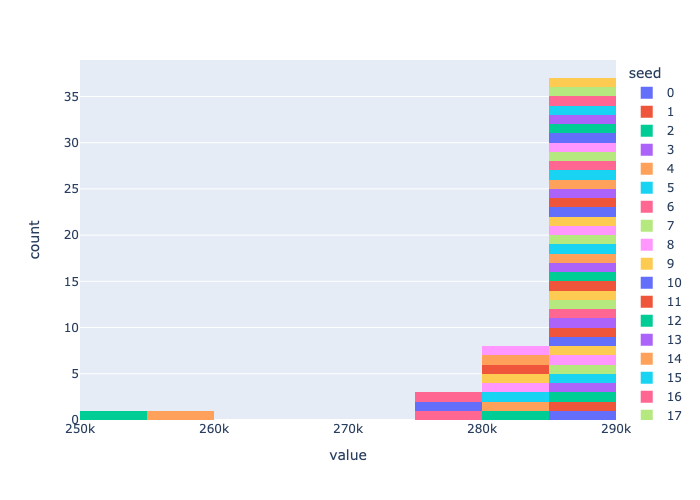
\includegraphics[width=\columnwidth]{assets/end-of-first-year-distribution.png}
\caption{A chart showing the balance over for 50 experiments (current OpenTTDLab )}
\label{fig:first-year}
\end{figure}

\begin{figure}[h]
\centering
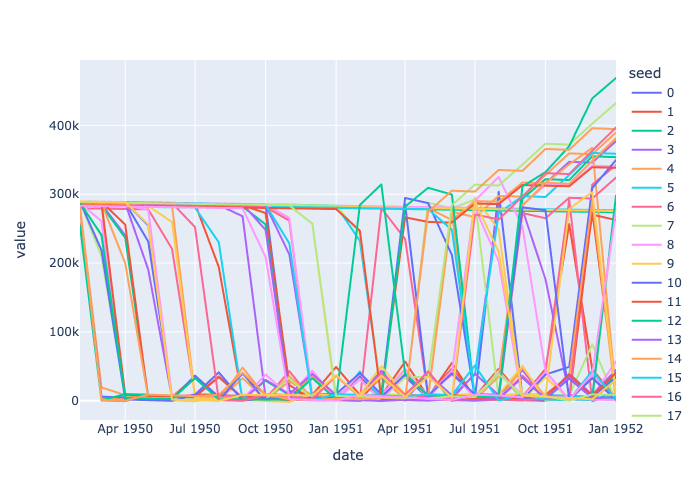
\includegraphics[width=\columnwidth]{assets/first-2-years.png}
\caption{A chart showing the balance over for 50 experiments (current OpenTTDLab )}
\label{fig:first-year}
\end{figure}

\begin{figure}[h]
\centering
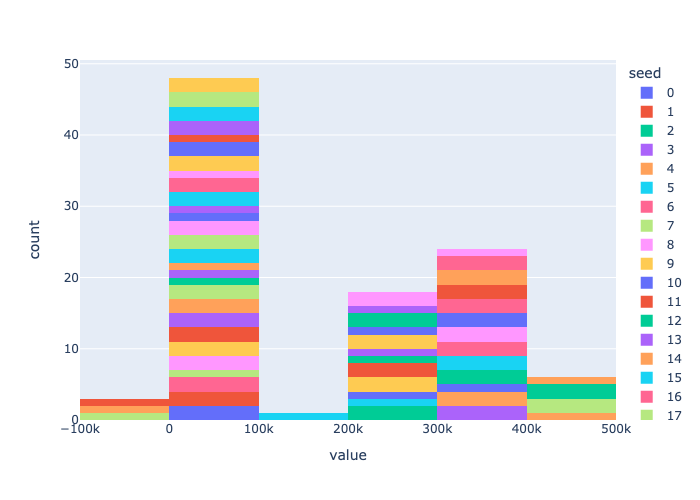
\includegraphics[width=\columnwidth]{assets/end-of-second-year-distribution.png}
\caption{A chart showing the balance over for 50 experiments (current OpenTTDLab )}
\label{fig:first-year}
\end{figure}

\begin{figure}[h]
\centering
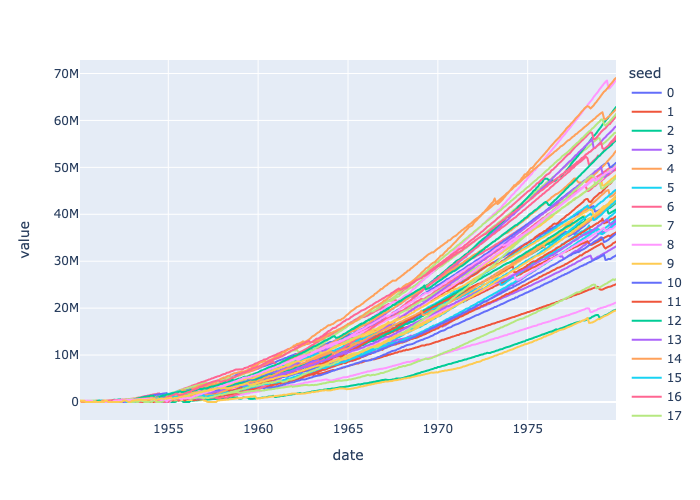
\includegraphics[width=\columnwidth]{assets/value-over-time-2.png}
\caption{A chart showing the balance over for 50 experiments (current OpenTTDLab )}
\label{fig:value-over-time}
\end{figure}

\begin{figure}[h]
\centering
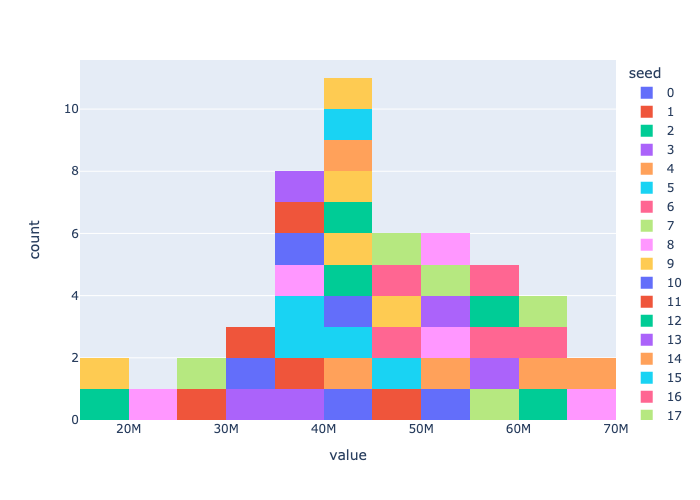
\includegraphics[width=\columnwidth]{assets/end-of-30th-year-distribution.png}
\caption{A chart showing the balance over for 50 experiments (current OpenTTDLab )}
\label{fig:first-year}
\end{figure}

\begin{figure}[h]
\centering
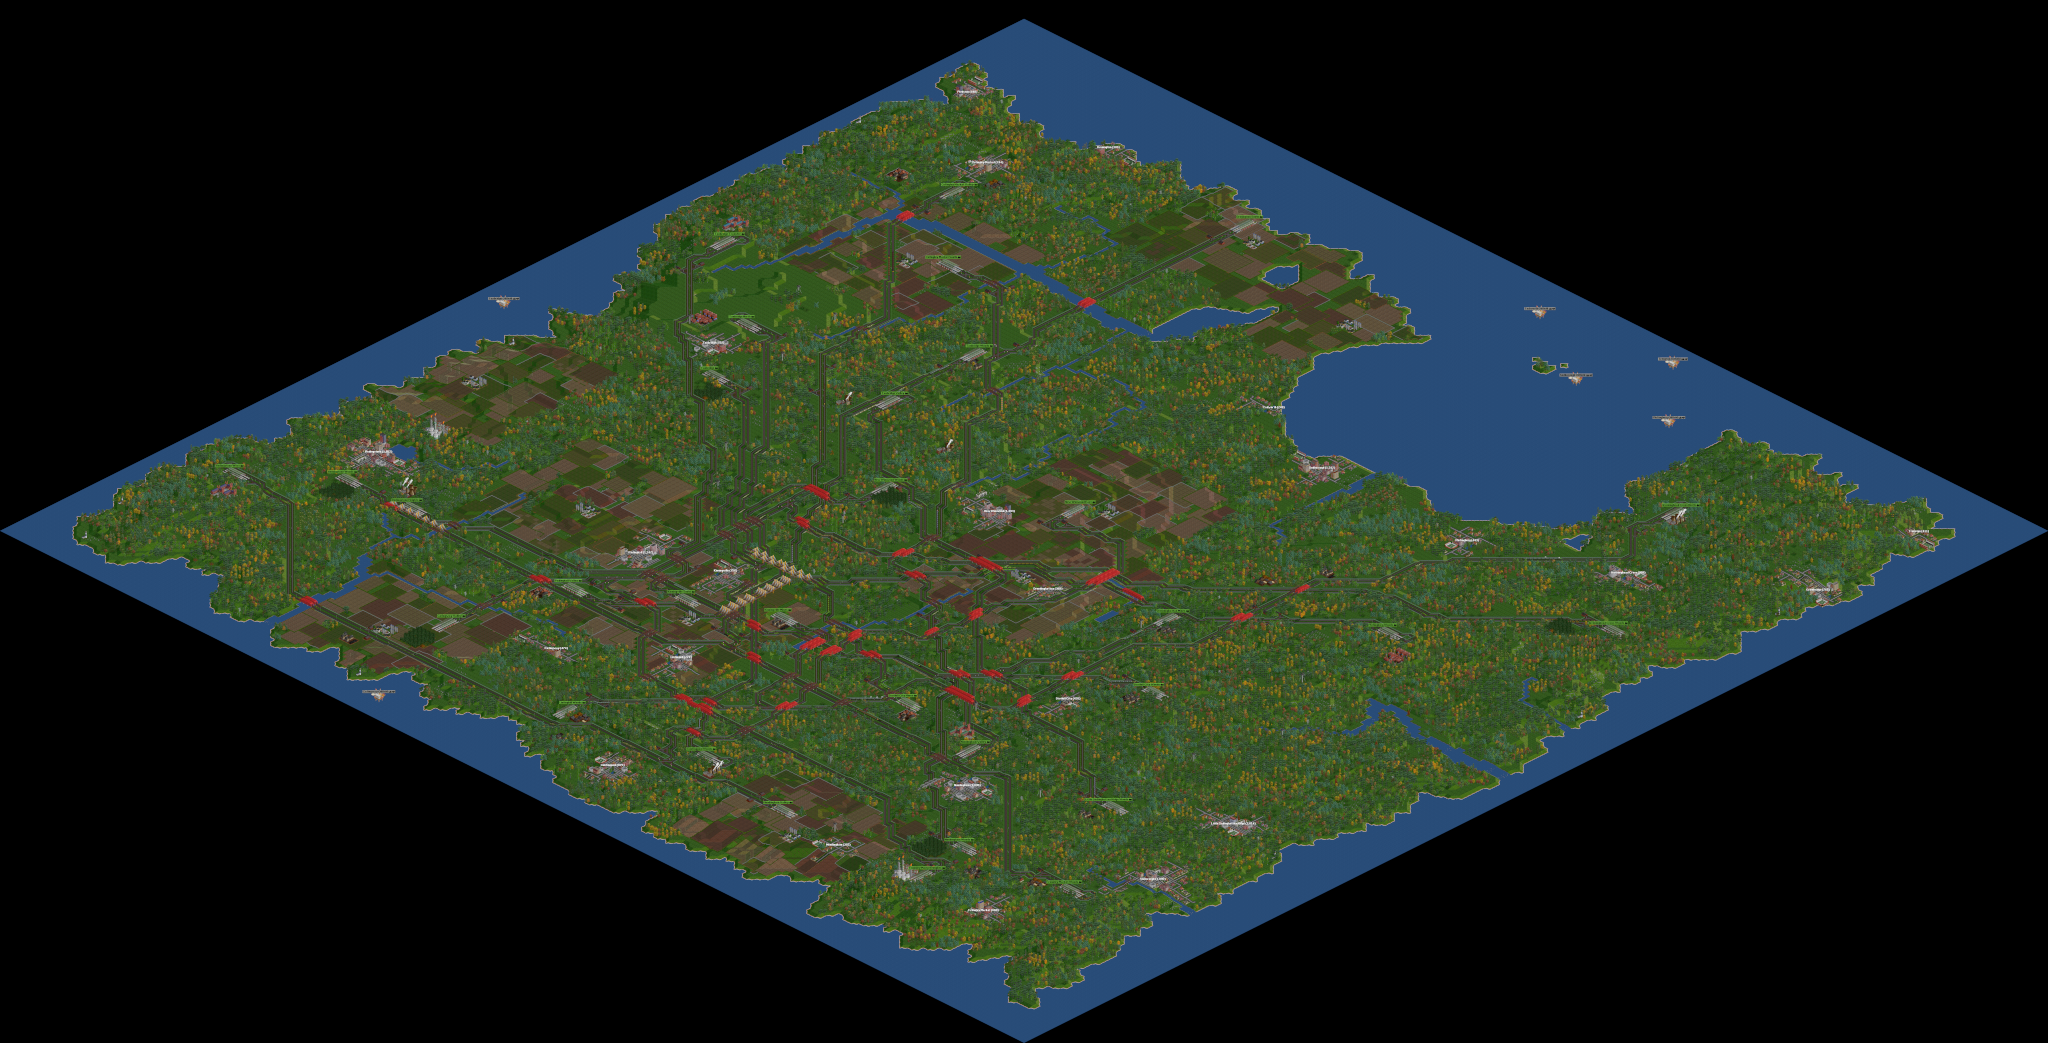
\includegraphics[width=\columnwidth]{assets/34_small.png}
\caption{Seed 34 - with the highest money at end}
\label{fig:openttd}
\end{figure}

\begin{figure}[h]
\centering
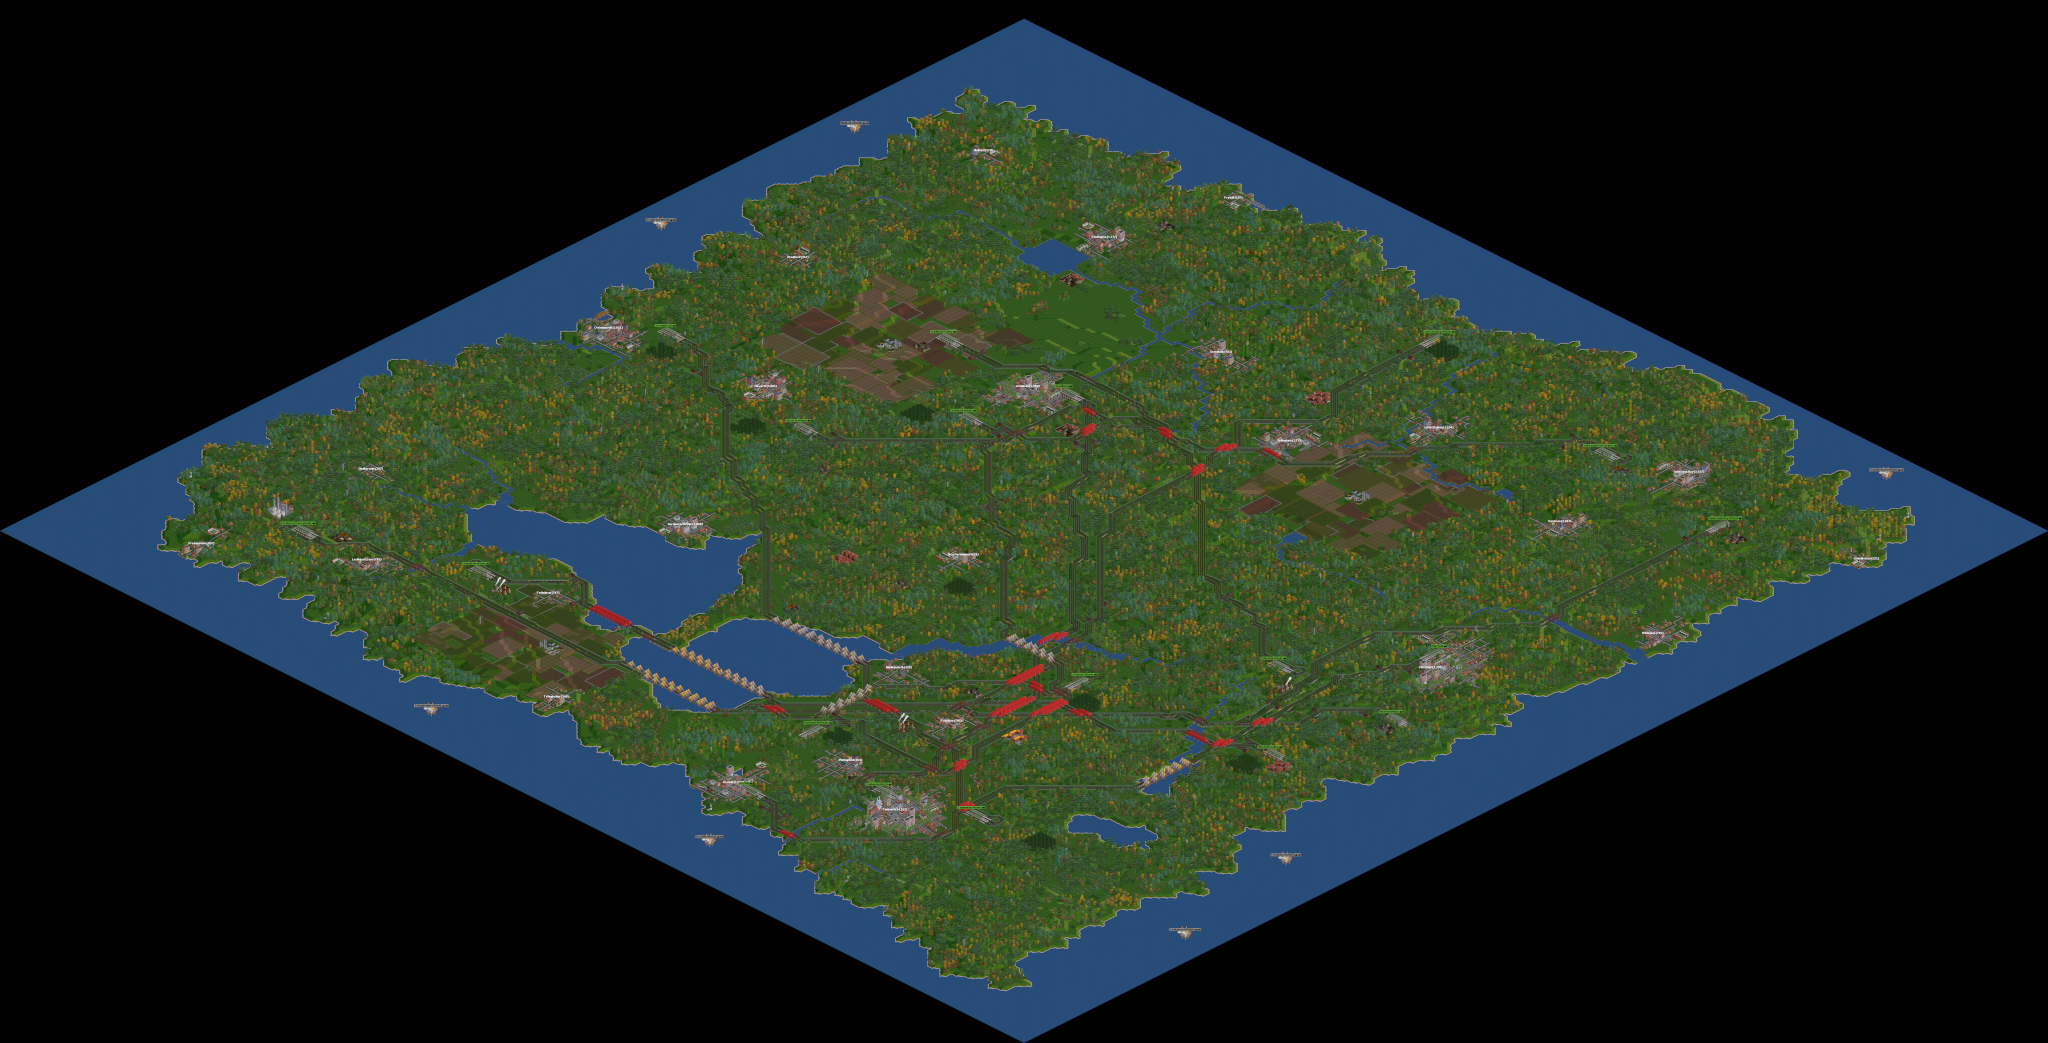
\includegraphics[width=\columnwidth]{assets/19_small.png}
\caption{Seed 19 - with the lowest money at end}
\label{fig:openttd}
\end{figure}

\begin{figure}[h]
\centering
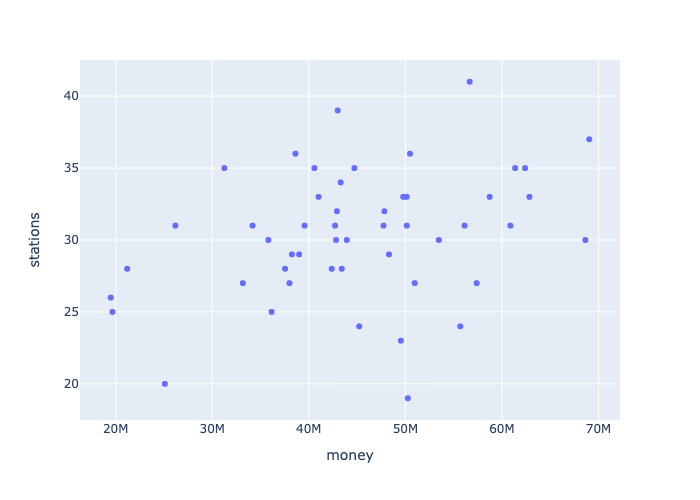
\includegraphics[width=\columnwidth]{assets/stations_vs_money.png}
\caption{Not much of a corrolation between stations and money!}
\label{fig:openttd}
\end{figure}

Bit of a "story" - starts off 300k. Then after a time there is a bi-modal distribution on money, then all the companies have have money in a normal-ish distribution.

Looks like the one with more stations/routes has more money? Can we corrolate stations with money?




------

\begin{figure}[h]
\centering
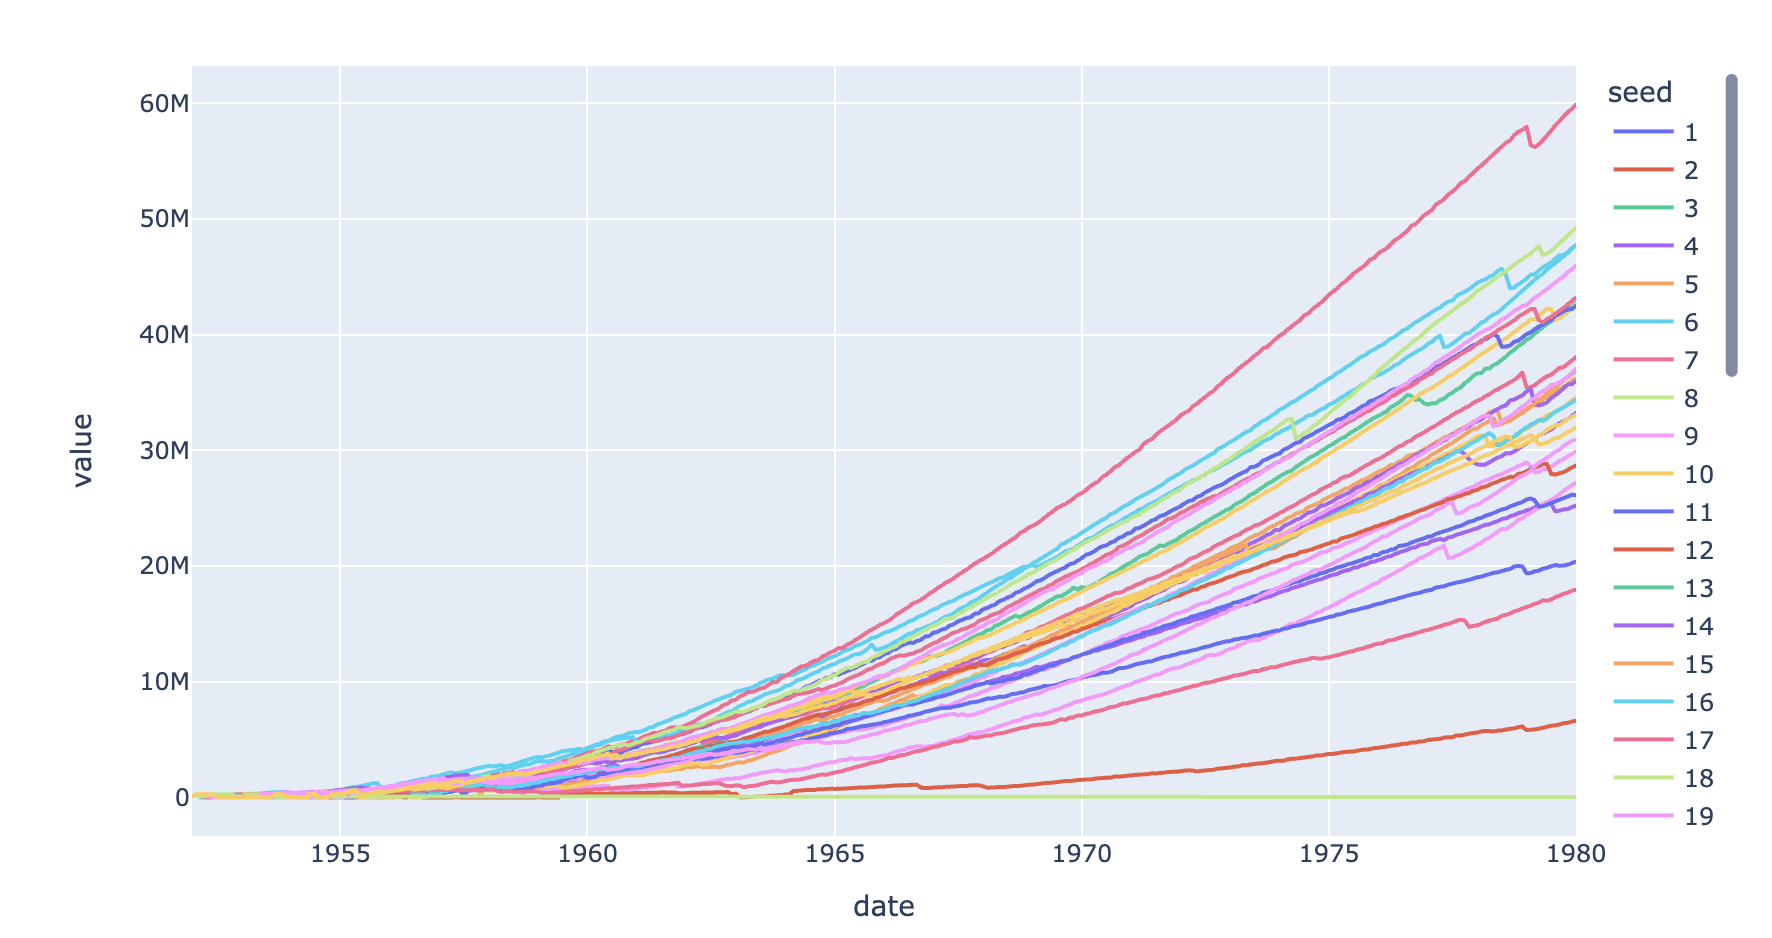
\includegraphics[width=\columnwidth]{assets/value-over-time.png}
\caption{A chart showing the balance over for 50 experiments (old version of OpenTTDLab - can't reproduce! Suspect because now AIs are started immediately, and so the random numbers are different? Will check on older OpenTTDLab)}
\label{fig:value-over-time}
\end{figure}







\chapter{Conclusion}

\begin{itemize}
\begin{item}
Maybe mention the link between this and testing here? Or should it be earlier?
\end{item}
\end{itemize}

The framework presented here allows experiments to be conducted with OpenTTD in a manner that is repeatable and reproducible. Reproducibility is up to the author's descriptions of the artefacts they created - they must be sufficient to recreate the artefacts, and so beyond the scope of the framework here. However, it should at least ease issues due to creating a similar enough experimental setup.

The exception are the version of the AI used - these do not appear to be versioned. However, potentially it could report on some sort of hash of the code of the AI.

Loads of further work. Two camps: developing OpenTTDLab reproducible: version stuff, action, file format to save for example? Parallelise, easier optimisation. User research as per EXAMPLE. But then using OpenTTDLab as well! Hopefully the results chapter will show it can be used to analyse existing AIs, develop new AIs in order to explore specific concepts, which in this case is risk/benefit trade off, and also exploring ways of optimising, er, something.

\chapter{Notes}

History

\begin{itemize}

\begin{item}
\cite{jackson1959learning} first business simulation game, US Air force MONOPOLOGS pretend to be inventory managers
\end{item}

\begin{item}
\cite{meijer2009organisation} - Studying supply chains using gaming simulation
\end{item}

\begin{item}
\cite{mayer2009gaming} - Defines simulation game as a game "experi(m)ent(i)al, rule-based, interactive environments, where players learn by taking actions and by experiencing their effects through feedback mechanisms that are deliberately built into and around the game"
\end{item}

\begin{item}
\cite{raghothama2013review} war gaming roots, policy analysis, business simulation games, studies on human cognition and behavior, training and pedagogical tools

Main point: simulation games particular suited for transportation research in general, and supply chain specifically because it's an emergent property

Some features of OpenTTD realistic, but this isn't exactly justified

Simutrans mentioned - described as not being realistic at all, but is extensible so could be

But similuation games not used for transportation

Gives lots of examples of simulation games used for research, but also mentions "Little attention has been paid to the validation of these simulation games."

(But: by and large here we're not concerning ourselves with validation)
\end{item}

\begin{item}
Basically have a list of a good range of how similuation games have been used.
\end{item}

\begin{item}
\cite{alderliesten2019maintrain} The simulation game itself used to try to get sympathy/understanding from passengers about delays
\end{item}

\begin{item}
\cite{cimellaro2016computational} - it lists OpenTTD alongside "real" simulators of cities in discussion for disaster reliance, with no particular mention that's it a game/for entertainment??
\end{item}

Repeatability


\begin{itemize}
\begin{item}
\cite{dalle2012reproducibility} in simulation in particular "many published works based on simulation still fail to meet the minimum conditions to ensure reproducibility" (and in my opinion the OpenTTD ones are no exception). And it gives some "levels" L1, L2, L3, L4 on how to judge "how" reproducbiel simulations are and highlights specific desirable details about simulations. I can probably judge some existing research using this, and compare to maybe output using my OpenTTDLab thing?

Hidden details that prevent reproducilibty (it cites another source for this)

I quite like this one! (TODO Check things that cite it especially)

"Goes beyond" reproducibility into traceability...

"– a simulator refers to a reusable simulation engine and its Application Programming Interface
(API); the engine is reusable for the simulation of many models and scenarios;" OpenTTDLab I think is the "missing" simulator??

"In simulation, not only the same sources of error
exist, but the system itself can be modeled incorrectly and be a source of error"

"Furthermore, as will be explained in greater details
in the next section, simulation has many applications that are not aimed toward producing science
and, therefore, do not necessarily require a reproducibility based on the source code availability."

"• manipulation errors: These errors result from the manual handling of some of the tasks in the simulation study work-flow."

OpenTTDLab I think addresses loads of the issues mentioned, in many of the ways it suggests.
\end{item}


\begin{item}
\cite{monks2019strengthening} - Checklist style "STRESS" guidelines. Strengthening the Reporting of Empirical Simulation Studies

It also has a review of lots of other guidelines for reproducible simulations

TODO: if going this way, reflect on the bits that OpenTTDLab does not do

"Agent-Based Simulation (ABS), Discrete-Event Simulation (DES) and System Dynamics (SD)." - er... OpenTTD is which of these??

"it is critical that author report the software version and build numbers" - this is for commercial software, but I would argue for Open Source as well
\end{item}

\begin{item}
Gass (1984) provides the earliest example of reporting guidelines for “computer based models”.
\end{item}
\end{itemize}

\end{itemize}


\bibliographystyle{plain}
\bibliography{mybibfile}


% You may delete everything from \appendix up to \end{document} if you don't need it.
\appendix

\chapter{Summary of data in OpenTTD save games}


Any appendices, including any required ethics information, should be included
after the references.

Markers do not have to consider appendices. Make sure that your contributions
are made clear in the main body of the dissertation (within the page limit).

\chapter{Documentation of OpenTTDLab}

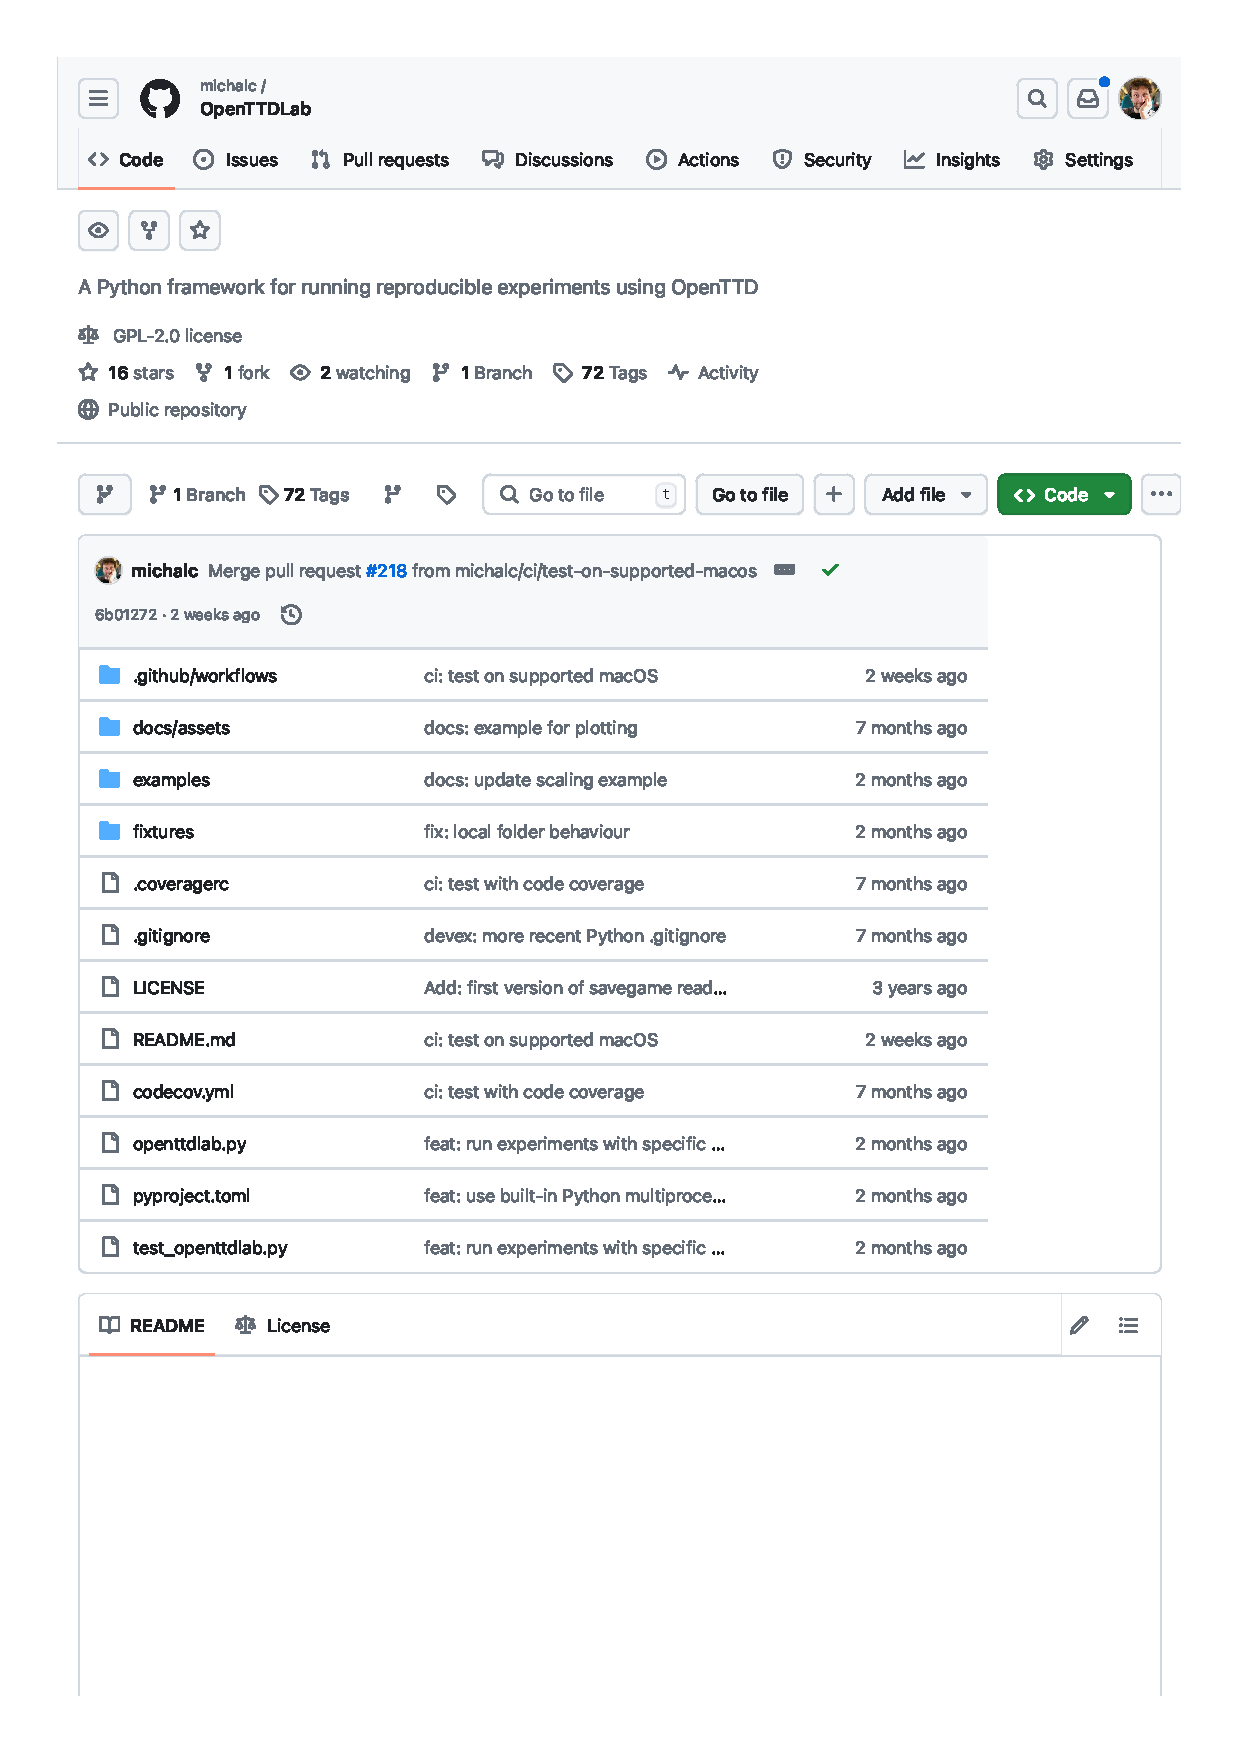
\includepdf[pages=-,scale=.8,pagecommand={}]{assets/openttdlab-github.pdf}

\chapter{Scaling experiments - Python code to run experiments}
\label{chapter:scaling-running-code}

The Python notebook used to generate results for the Scaling experiments of XX is below. This latest version is also available at \url{https://github.com/michalc/openttd-msc-dissertation/blob/main/notebooks/01_scaling_01_run_experiment.ipynb}

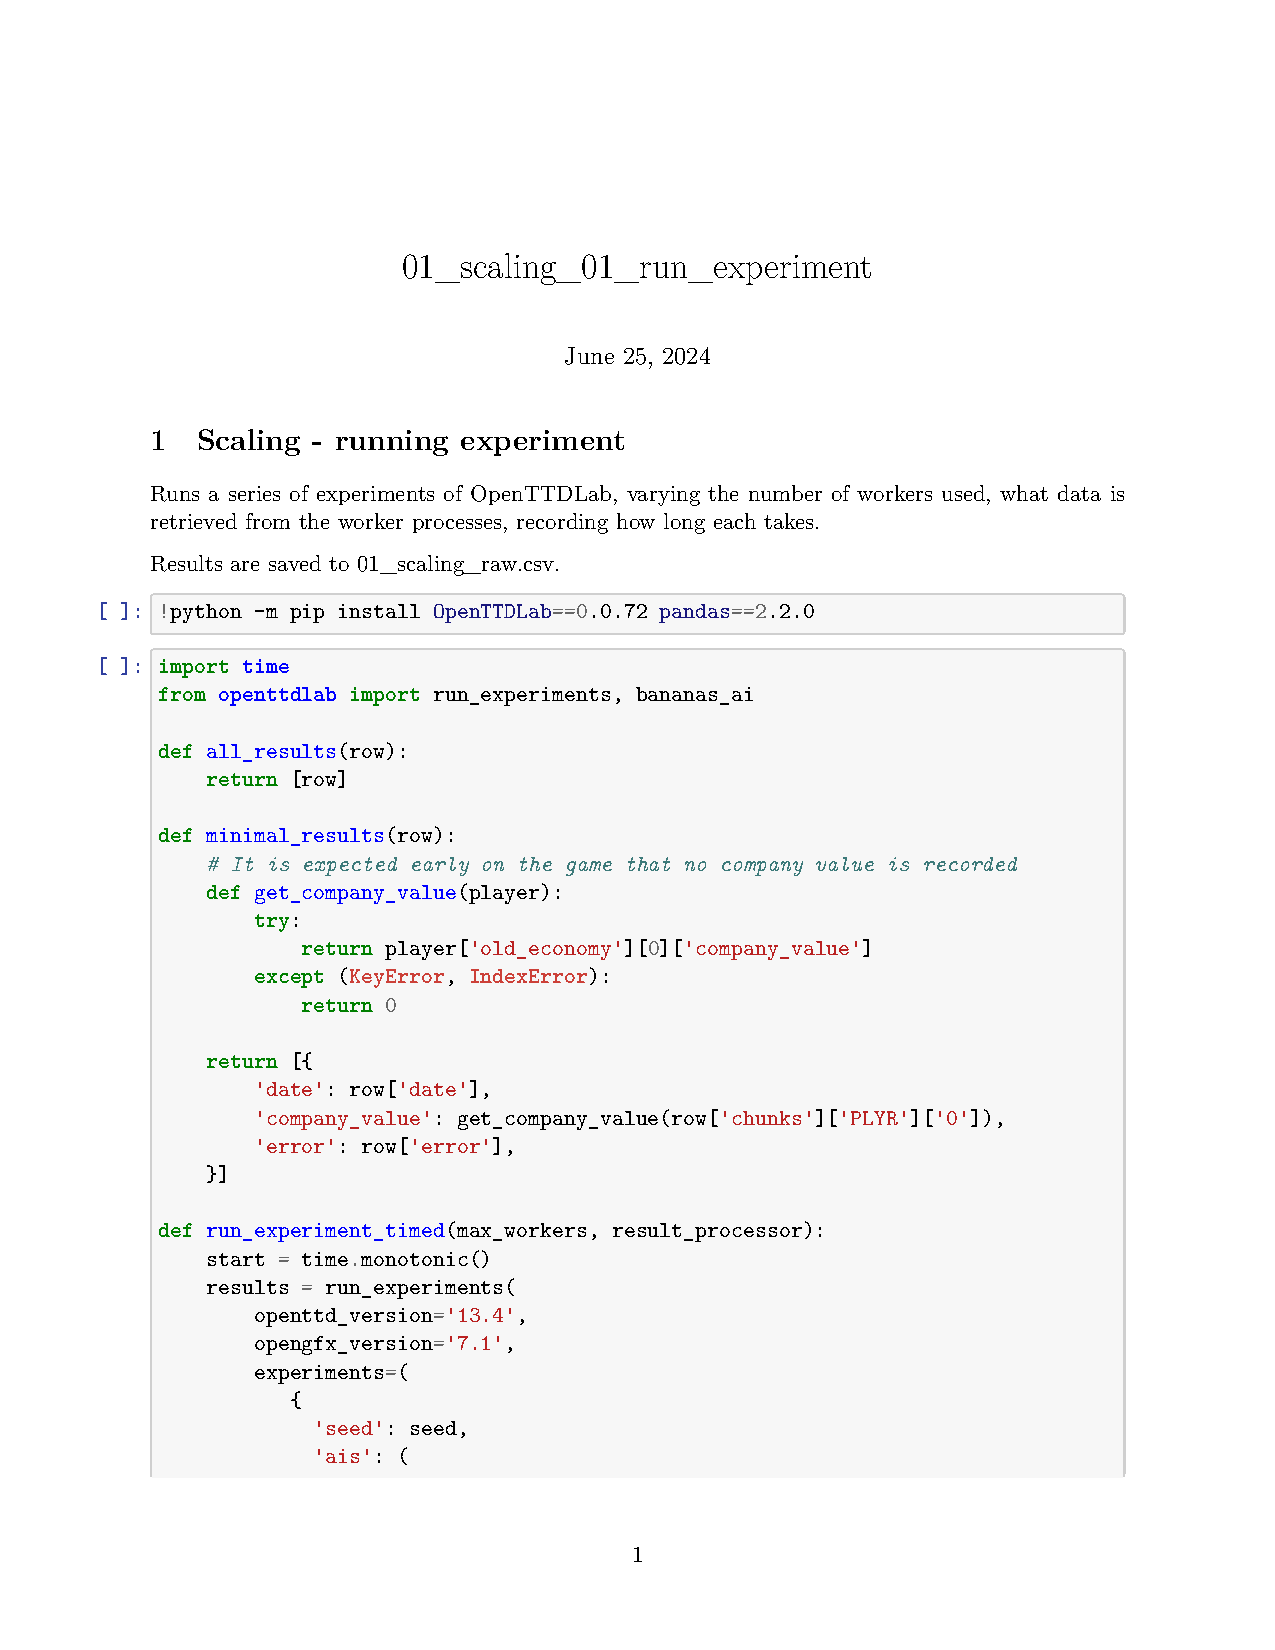
\includepdf[pages=-,scale=.8,pagecommand={}]{notebooks/01_scaling_01_run_experiment.pdf}

\chapter{Scaling experiments - Python code to analyse results}
\label{chapter:scaling-analyis-code}

The Python notebook used to analyse results for the Scaling experiments of XX is below. This latest version is also available at \url{https://github.com/michalc/openttd-msc-dissertation/blob/main/notebooks/01_scaling_02_analyse_results.ipynb}

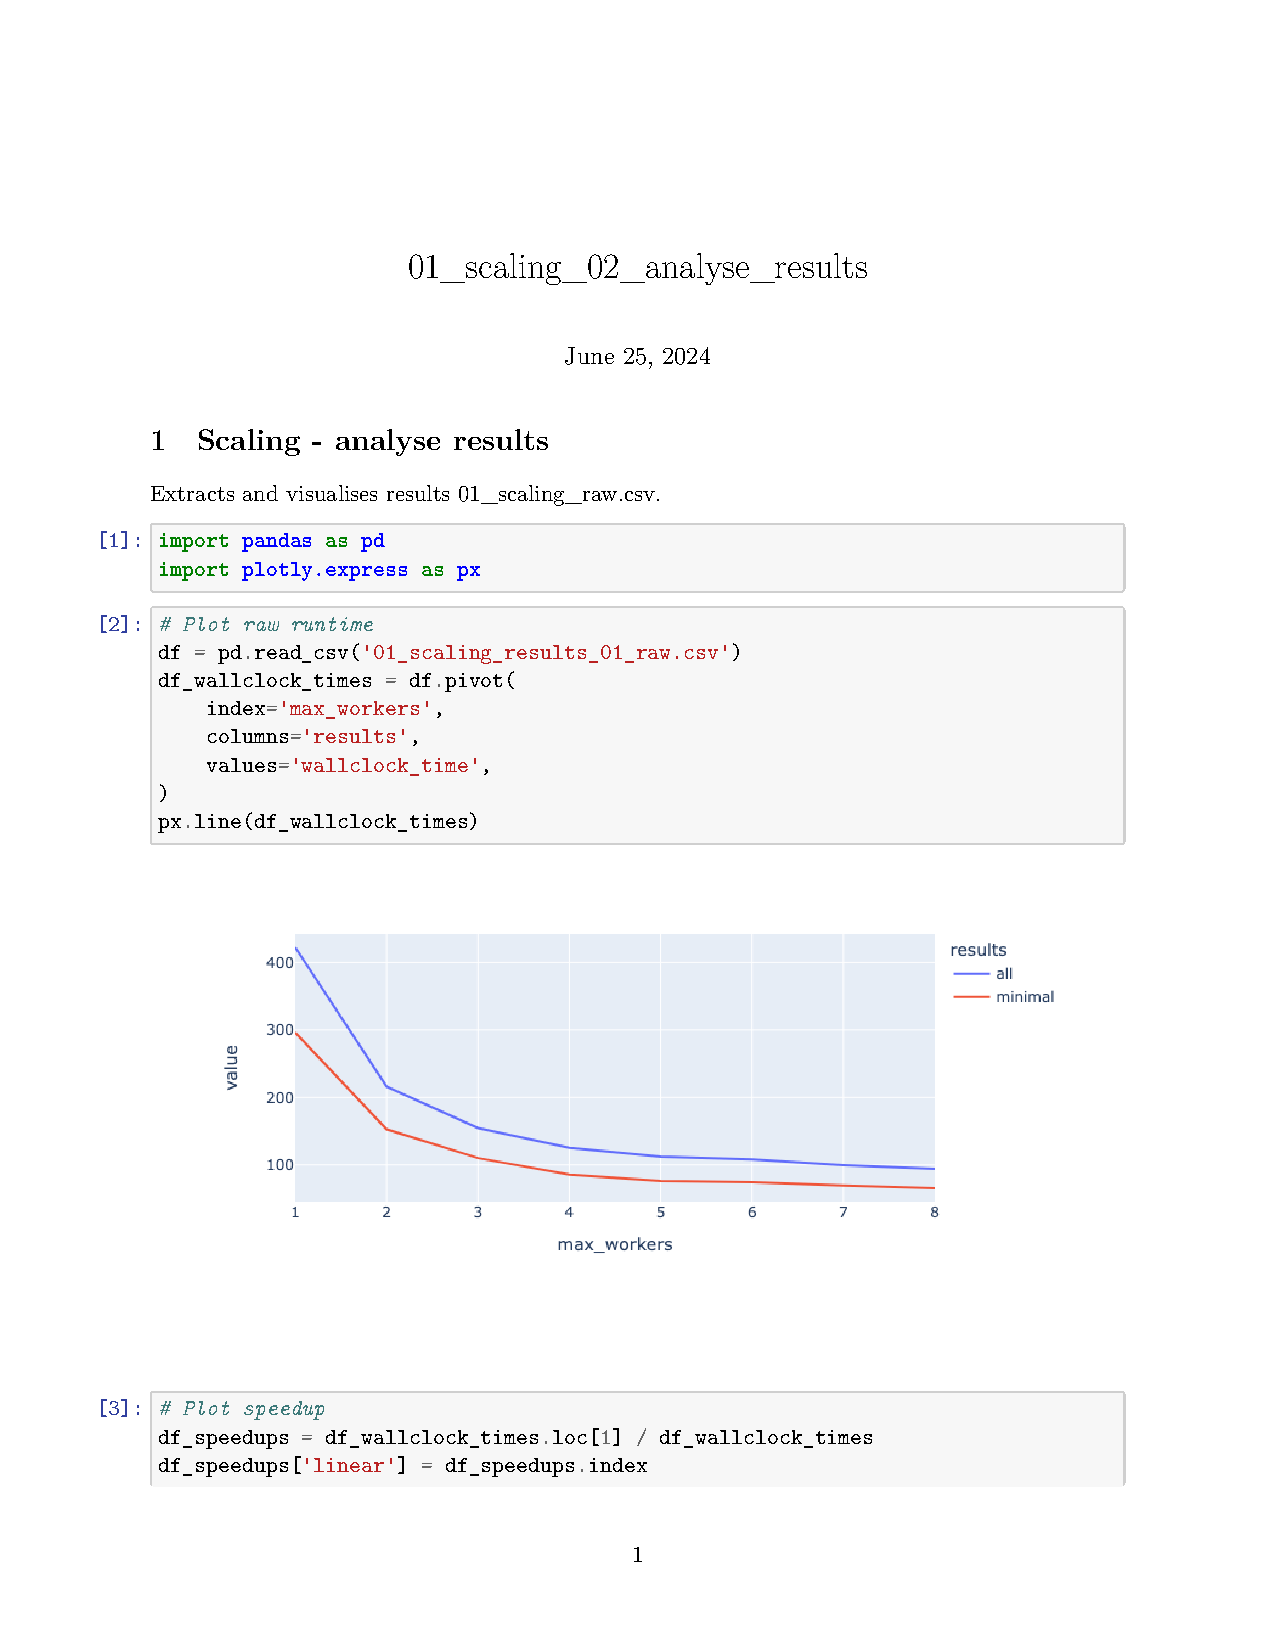
\includepdf[pages=-,scale=.8,pagecommand={}]{notebooks/01_scaling_02_analyse_results.pdf}


\end{document}
